\documentclass[twoside]{book}

% Packages required by doxygen
\usepackage{fixltx2e}
\usepackage{calc}
\usepackage{doxygen}
\usepackage[export]{adjustbox} % also loads graphicx
\usepackage{graphicx}
\usepackage[utf8]{inputenc}
\usepackage{makeidx}
\usepackage{multicol}
\usepackage{multirow}
\PassOptionsToPackage{warn}{textcomp}
\usepackage{textcomp}
\usepackage[nointegrals]{wasysym}
\usepackage[table]{xcolor}

% Font selection
\usepackage[T1]{fontenc}
\usepackage[scaled=.90]{helvet}
\usepackage{courier}
\usepackage{amssymb}
\usepackage{sectsty}
\renewcommand{\familydefault}{\sfdefault}
\allsectionsfont{%
  \fontseries{bc}\selectfont%
  \color{darkgray}%
}
\renewcommand{\DoxyLabelFont}{%
  \fontseries{bc}\selectfont%
  \color{darkgray}%
}
\newcommand{\+}{\discretionary{\mbox{\scriptsize$\hookleftarrow$}}{}{}}

% Page & text layout
\usepackage{geometry}
\geometry{%
  a4paper,%
  top=2.5cm,%
  bottom=2.5cm,%
  left=2.5cm,%
  right=2.5cm%
}
\tolerance=750
\hfuzz=15pt
\hbadness=750
\setlength{\emergencystretch}{15pt}
\setlength{\parindent}{0cm}
\setlength{\parskip}{3ex plus 2ex minus 2ex}
\makeatletter
\renewcommand{\paragraph}{%
  \@startsection{paragraph}{4}{0ex}{-1.0ex}{1.0ex}{%
    \normalfont\normalsize\bfseries\SS@parafont%
  }%
}
\renewcommand{\subparagraph}{%
  \@startsection{subparagraph}{5}{0ex}{-1.0ex}{1.0ex}{%
    \normalfont\normalsize\bfseries\SS@subparafont%
  }%
}
\makeatother

% Headers & footers
\usepackage{fancyhdr}
\pagestyle{fancyplain}
\fancyhead[LE]{\fancyplain{}{\bfseries\thepage}}
\fancyhead[CE]{\fancyplain{}{}}
\fancyhead[RE]{\fancyplain{}{\bfseries\leftmark}}
\fancyhead[LO]{\fancyplain{}{\bfseries\rightmark}}
\fancyhead[CO]{\fancyplain{}{}}
\fancyhead[RO]{\fancyplain{}{\bfseries\thepage}}
\fancyfoot[LE]{\fancyplain{}{}}
\fancyfoot[CE]{\fancyplain{}{}}
\fancyfoot[RE]{\fancyplain{}{\bfseries\scriptsize Generated by Doxygen }}
\fancyfoot[LO]{\fancyplain{}{\bfseries\scriptsize Generated by Doxygen }}
\fancyfoot[CO]{\fancyplain{}{}}
\fancyfoot[RO]{\fancyplain{}{}}
\renewcommand{\footrulewidth}{0.4pt}
\renewcommand{\chaptermark}[1]{%
  \markboth{#1}{}%
}
\renewcommand{\sectionmark}[1]{%
  \markright{\thesection\ #1}%
}

% Indices & bibliography
\usepackage{natbib}
\usepackage[titles]{tocloft}
\setcounter{tocdepth}{3}
\setcounter{secnumdepth}{5}
\makeindex

% Custom commands
\newcommand{\clearemptydoublepage}{%
  \newpage{\pagestyle{empty}\cleardoublepage}%
}

\usepackage{caption}
\captionsetup{labelsep=space,justification=centering,font={bf},singlelinecheck=off,skip=4pt,position=top}

%===== C O N T E N T S =====

\begin{document}

% Titlepage & ToC
\pagenumbering{alph}
\begin{titlepage}
\vspace*{7cm}
\begin{center}%
{\Large Cookie Engine }\\
\vspace*{1cm}
{\large Generated by Doxygen 1.8.13}\\
\end{center}
\end{titlepage}
\clearemptydoublepage
\pagenumbering{roman}
\tableofcontents
\clearemptydoublepage
\pagenumbering{arabic}

%--- Begin generated contents ---
\chapter{Games Programming Level 6 -\/ Game Engine Programming (Cookie Engine)}
\label{index}\hypertarget{index_sec_intro}{}\section{Introduction}\label{index_sec_intro}
Welcome to the documentation for Cookie Engine! This project was created on the Bournemouth University Game Programming course for the Game Engine Programming unit. This documentation covers the setup to build the project from the source for running on a Windows 10 PC as well as documentation for all classes.\hypertarget{index_sec_running}{}\section{Install}\label{index_sec_running}

\begin{DoxyEnumerate}
\item Load the solution in Microsoft Visual Studio 2017 or later.
\item Select the x86 Solution Platform.
\item Select the Release Solution Configuration.
\item Build the project
\item You should now have a Cookie\+Eng.\+lib file!
\end{DoxyEnumerate}\hypertarget{index_sec_use}{}\section{Use}\label{index_sec_use}
To use the engine, first include the Cookie\+Eng.\+lib file and corresponding headers to your project 
\chapter{Class Index}
\section{Class List}
Here are the classes, structs, unions and interfaces with brief descriptions\+:\begin{DoxyCompactList}
\item\contentsline{section}{\hyperlink{class_cookie_eng_1_1_components_1_1_bounding_box}{Cookie\+Eng\+::\+Components\+::\+Bounding\+Box} \\*An axis aligned bounding box represented by the two minimum and maximum corners }{\pageref{class_cookie_eng_1_1_components_1_1_bounding_box}}{}
\item\contentsline{section}{\hyperlink{class_cookie_eng_1_1_object_1_1_camera}{Cookie\+Eng\+::\+Object\+::\+Camera} \\*Contains the data for the representation of a perspective camera }{\pageref{class_cookie_eng_1_1_object_1_1_camera}}{}
\item\contentsline{section}{\hyperlink{class_cookie_eng_1_1_e_c_s_1_1_component}{Cookie\+Eng\+::\+E\+C\+S\+::\+Component} \\*The component base class }{\pageref{class_cookie_eng_1_1_e_c_s_1_1_component}}{}
\item\contentsline{section}{\hyperlink{class_cookie_eng_1_1_cookie_core}{Cookie\+Eng\+::\+Cookie\+Core} \\*The engine core class }{\pageref{class_cookie_eng_1_1_cookie_core}}{}
\item\contentsline{section}{\hyperlink{class_cookie_eng_1_1_e_c_s_1_1_entity}{Cookie\+Eng\+::\+E\+C\+S\+::\+Entity} \\*Holds together a group of components that are unique of each other }{\pageref{class_cookie_eng_1_1_e_c_s_1_1_entity}}{}
\item\contentsline{section}{\hyperlink{class_cookie_eng_1_1_services_1_1_file_manager}{Cookie\+Eng\+::\+Services\+::\+File\+Manager} \\*A Manager Class that handles the loading of files either synchronously or asynchronously }{\pageref{class_cookie_eng_1_1_services_1_1_file_manager}}{}
\item\contentsline{section}{\hyperlink{class_cookie_eng_1_1_graphics_1_1_frame_buffer}{Cookie\+Eng\+::\+Graphics\+::\+Frame\+Buffer} \\*Abstraction of an Open\+GL \hyperlink{class_cookie_eng_1_1_graphics_1_1_frame_buffer}{Frame\+Buffer} }{\pageref{class_cookie_eng_1_1_graphics_1_1_frame_buffer}}{}
\item\contentsline{section}{\hyperlink{class_cookie_eng_1_1_messaging_1_1_i_message_handler}{Cookie\+Eng\+::\+Messaging\+::\+I\+Message\+Handler} \\*The base class for engine objects that require the ability to receive messages }{\pageref{class_cookie_eng_1_1_messaging_1_1_i_message_handler}}{}
\item\contentsline{section}{\hyperlink{class_cookie_eng_1_1_services_1_1_initialiser}{Cookie\+Eng\+::\+Services\+::\+Initialiser} \\*Initialisation for external libraries }{\pageref{class_cookie_eng_1_1_services_1_1_initialiser}}{}
\item\contentsline{section}{\hyperlink{class_cookie_eng_1_1_input_1_1_input_manager}{Cookie\+Eng\+::\+Input\+::\+Input\+Manager} }{\pageref{class_cookie_eng_1_1_input_1_1_input_manager}}{}
\item\contentsline{section}{\hyperlink{class_cookie_eng_1_1_input_1_1_keyboard_1_1_key}{Cookie\+Eng\+::\+Input\+::\+Keyboard\+::\+Key} \\*Contains a key\textquotesingle{}s state }{\pageref{class_cookie_eng_1_1_input_1_1_keyboard_1_1_key}}{}
\item\contentsline{section}{\hyperlink{class_cookie_eng_1_1_input_1_1_keyboard_1_1_keyboard}{Cookie\+Eng\+::\+Input\+::\+Keyboard\+::\+Keyboard} \\*A keyboard class that handles the state of various keys }{\pageref{class_cookie_eng_1_1_input_1_1_keyboard_1_1_keyboard}}{}
\item\contentsline{section}{\hyperlink{class_cookie_eng_1_1_resources_1_1_material}{Cookie\+Eng\+::\+Resources\+::\+Material} \\*A material that can be used for rendering }{\pageref{class_cookie_eng_1_1_resources_1_1_material}}{}
\item\contentsline{section}{\hyperlink{struct_cookie_eng_1_1_resources_1_1_mesh}{Cookie\+Eng\+::\+Resources\+::\+Mesh} \\*Data required for a raw \hyperlink{struct_cookie_eng_1_1_resources_1_1_mesh}{Mesh} }{\pageref{struct_cookie_eng_1_1_resources_1_1_mesh}}{}
\item\contentsline{section}{\hyperlink{class_cookie_eng_1_1_messaging_1_1_message}{Cookie\+Eng\+::\+Messaging\+::\+Message} \\*A \hyperlink{class_cookie_eng_1_1_messaging_1_1_message}{Message} for passing around the engine }{\pageref{class_cookie_eng_1_1_messaging_1_1_message}}{}
\item\contentsline{section}{\hyperlink{class_cookie_eng_1_1_services_1_1_message_queue}{Cookie\+Eng\+::\+Services\+::\+Message\+Queue} \\*A queue for distributing messages to Observers }{\pageref{class_cookie_eng_1_1_services_1_1_message_queue}}{}
\item\contentsline{section}{\hyperlink{class_cookie_eng_1_1_data_1_1_primative_generator}{Cookie\+Eng\+::\+Data\+::\+Primative\+Generator} }{\pageref{class_cookie_eng_1_1_data_1_1_primative_generator}}{}
\item\contentsline{section}{\hyperlink{struct_cookie_eng_1_1_data_1_1_ray}{Cookie\+Eng\+::\+Data\+::\+Ray} \\*A ray represented by an origin point and a direction for an infinite distance }{\pageref{struct_cookie_eng_1_1_data_1_1_ray}}{}
\item\contentsline{section}{\hyperlink{class_cookie_eng_1_1_components_1_1_renderable}{Cookie\+Eng\+::\+Components\+::\+Renderable} \\*An Component for providing the data needed to render to the screen }{\pageref{class_cookie_eng_1_1_components_1_1_renderable}}{}
\item\contentsline{section}{\hyperlink{class_cookie_eng_1_1_graphics_1_1_renderer}{Cookie\+Eng\+::\+Graphics\+::\+Renderer} \\*An Open\+GL \hyperlink{class_cookie_eng_1_1_graphics_1_1_renderer}{Renderer} }{\pageref{class_cookie_eng_1_1_graphics_1_1_renderer}}{}
\item\contentsline{section}{\hyperlink{class_cookie_eng_1_1_resources_1_1_resource}{Cookie\+Eng\+::\+Resources\+::\+Resource} \\*A base class for any engine resources (stuff that can be loaded) }{\pageref{class_cookie_eng_1_1_resources_1_1_resource}}{}
\item\contentsline{section}{\hyperlink{class_cookie_eng_1_1_res_mgmt_1_1_resource_loader}{Cookie\+Eng\+::\+Res\+Mgmt\+::\+Resource\+Loader} \\*Loads a list of resources from a .lvl file }{\pageref{class_cookie_eng_1_1_res_mgmt_1_1_resource_loader}}{}
\item\contentsline{section}{\hyperlink{class_cookie_eng_1_1_res_mgmt_1_1_resource_manager}{Cookie\+Eng\+::\+Res\+Mgmt\+::\+Resource\+Manager} \\*A Singleton for handling the storage of resources }{\pageref{class_cookie_eng_1_1_res_mgmt_1_1_resource_manager}}{}
\item\contentsline{section}{\hyperlink{class_cookie_eng_1_1_scene_1_1_scene}{Cookie\+Eng\+::\+Scene\+::\+Scene} \\*A level representation containing entities }{\pageref{class_cookie_eng_1_1_scene_1_1_scene}}{}
\item\contentsline{section}{\hyperlink{class_cookie_eng_1_1_services_1_1_service_container}{Cookie\+Eng\+::\+Services\+::\+Service\+Container} \\*The \hyperlink{class_cookie_eng_1_1_services_1_1_service_container}{Service\+Container} acts as a container for services that can be located by the \hyperlink{class_cookie_eng_1_1_services_1_1_service_locator}{Service\+Locator} }{\pageref{class_cookie_eng_1_1_services_1_1_service_container}}{}
\item\contentsline{section}{\hyperlink{class_cookie_eng_1_1_services_1_1_service_locator}{Cookie\+Eng\+::\+Services\+::\+Service\+Locator} \\*Works as an interface to the managers and services provided by the engine }{\pageref{class_cookie_eng_1_1_services_1_1_service_locator}}{}
\item\contentsline{section}{\hyperlink{class_cookie_eng_1_1_graphics_1_1_shader}{Cookie\+Eng\+::\+Graphics\+::\+Shader} \\*Abstracted Open\+GL \hyperlink{class_cookie_eng_1_1_graphics_1_1_shader}{Shader} }{\pageref{class_cookie_eng_1_1_graphics_1_1_shader}}{}
\item\contentsline{section}{\hyperlink{class_cookie_eng_1_1_resources_1_1_shader_program}{Cookie\+Eng\+::\+Resources\+::\+Shader\+Program} \\*Abstracted Open\+GL Program }{\pageref{class_cookie_eng_1_1_resources_1_1_shader_program}}{}
\item\contentsline{section}{\hyperlink{class_cookie_eng_1_1_resources_1_1_texture}{Cookie\+Eng\+::\+Resources\+::\+Texture} \\*An abstraction of an Open\+GL \hyperlink{class_cookie_eng_1_1_resources_1_1_texture}{Texture} }{\pageref{class_cookie_eng_1_1_resources_1_1_texture}}{}
\item\contentsline{section}{\hyperlink{class_cookie_eng_1_1_threads_1_1_thread_pool}{Cookie\+Eng\+::\+Threads\+::\+Thread\+Pool} }{\pageref{class_cookie_eng_1_1_threads_1_1_thread_pool}}{}
\item\contentsline{section}{\hyperlink{class_cookie_eng_1_1_utilities_1_1_timer}{Cookie\+Eng\+::\+Utilities\+::\+Timer} \\*A timer that can time from start to an abitrary point }{\pageref{class_cookie_eng_1_1_utilities_1_1_timer}}{}
\item\contentsline{section}{\hyperlink{struct_cookie_eng_1_1_utilities_1_1_times}{Cookie\+Eng\+::\+Utilities\+::\+Times} \\*Holds engine time values }{\pageref{struct_cookie_eng_1_1_utilities_1_1_times}}{}
\item\contentsline{section}{\hyperlink{class_cookie_eng_1_1_components_1_1_transform}{Cookie\+Eng\+::\+Components\+::\+Transform} \\*A \hyperlink{class_cookie_eng_1_1_components_1_1_transform}{Transform} Component }{\pageref{class_cookie_eng_1_1_components_1_1_transform}}{}
\item\contentsline{section}{\hyperlink{struct_cookie_eng_1_1_object_1_1u___camera_data}{Cookie\+Eng\+::\+Object\+::u\+\_\+\+Camera\+Data} \\*The C\+PU side uniform block for camera view and projection matrices }{\pageref{struct_cookie_eng_1_1_object_1_1u___camera_data}}{}
\item\contentsline{section}{\hyperlink{class_cookie_eng_1_1_utilities_1_1_utils_float}{Cookie\+Eng\+::\+Utilities\+::\+Utils\+Float} }{\pageref{class_cookie_eng_1_1_utilities_1_1_utils_float}}{}
\item\contentsline{section}{\hyperlink{class_cookie_eng_1_1_utilities_1_1_utils_str}{Cookie\+Eng\+::\+Utilities\+::\+Utils\+Str} \\*String Utilities }{\pageref{class_cookie_eng_1_1_utilities_1_1_utils_str}}{}
\item\contentsline{section}{\hyperlink{struct_cookie_eng_1_1_data_1_1_vertex}{Cookie\+Eng\+::\+Data\+::\+Vertex} \\*A vertex in 3D space }{\pageref{struct_cookie_eng_1_1_data_1_1_vertex}}{}
\item\contentsline{section}{\hyperlink{class_cookie_eng_1_1_graphics_1_1_vertex_array}{Cookie\+Eng\+::\+Graphics\+::\+Vertex\+Array} \\*Absraction of an Open\+GL Vertex Array Object (V\+AO) }{\pageref{class_cookie_eng_1_1_graphics_1_1_vertex_array}}{}
\item\contentsline{section}{\hyperlink{class_cookie_eng_1_1_graphics_1_1_vertex_buffer}{Cookie\+Eng\+::\+Graphics\+::\+Vertex\+Buffer} \\*An abstraction of an Open\+GL Vertex Bufer Object (V\+BO) }{\pageref{class_cookie_eng_1_1_graphics_1_1_vertex_buffer}}{}
\item\contentsline{section}{\hyperlink{struct_cookie_eng_1_1_graphics_1_1_vertex_buffer_element}{Cookie\+Eng\+::\+Graphics\+::\+Vertex\+Buffer\+Element} \\*Represents an element of a layout of data stored in a V\+AO }{\pageref{struct_cookie_eng_1_1_graphics_1_1_vertex_buffer_element}}{}
\item\contentsline{section}{\hyperlink{class_cookie_eng_1_1_graphics_1_1_vertex_buffer_layout}{Cookie\+Eng\+::\+Graphics\+::\+Vertex\+Buffer\+Layout} \\*Abstraction of the layout of a V\+BO }{\pageref{class_cookie_eng_1_1_graphics_1_1_vertex_buffer_layout}}{}
\item\contentsline{section}{\hyperlink{class_cookie_eng_1_1_window}{Cookie\+Eng\+::\+Window} \\*An abstraction of the S\+DL \hyperlink{class_cookie_eng_1_1_window}{Window} class which can be used to create a window for Open\+GL rendering }{\pageref{class_cookie_eng_1_1_window}}{}
\end{DoxyCompactList}

\chapter{Class Documentation}
\hypertarget{class_cookie_eng_1_1_services_1_1_file_manager}{}\section{Cookie\+Eng\+:\+:Services\+:\+:File\+Manager Class Reference}
\label{class_cookie_eng_1_1_services_1_1_file_manager}\index{Cookie\+Eng\+::\+Services\+::\+File\+Manager@{Cookie\+Eng\+::\+Services\+::\+File\+Manager}}


A Manager Class that handles the loading of files either synchronously or asynchronously.  




{\ttfamily \#include $<$File\+Manager.\+h$>$}

\subsection*{Public Member Functions}
\begin{DoxyCompactItemize}
\item 
\hyperlink{class_cookie_eng_1_1_services_1_1_file_manager_a3ff15b868df81ba7d9964382f6474ef5}{File\+Manager} ()
\begin{DoxyCompactList}\small\item\em The \hyperlink{class_cookie_eng_1_1_services_1_1_file_manager}{File\+Manager} Constructor. \end{DoxyCompactList}\item 
\hyperlink{class_cookie_eng_1_1_services_1_1_file_manager_a51e133f4fd86a874129a63be191b91ba}{$\sim$\+File\+Manager} ()
\begin{DoxyCompactList}\small\item\em The \hyperlink{class_cookie_eng_1_1_services_1_1_file_manager}{File\+Manager} Destructor. \end{DoxyCompactList}\item 
std\+::string \hyperlink{class_cookie_eng_1_1_services_1_1_file_manager_a744bde422e66fcfbfcc379a21ae90500}{load\+Text\+File} (std\+::string \+\_\+filepath)
\begin{DoxyCompactList}\small\item\em Synchronous loading of text files. \end{DoxyCompactList}\item 
std\+::string \hyperlink{class_cookie_eng_1_1_services_1_1_file_manager_abf50a7b6eb9fa88a9557254acbd2d9cc}{load\+Text\+File\+A\+Sync} (std\+::string \+\_\+filepath)
\begin{DoxyCompactList}\small\item\em Asynchronous loading of text files. \end{DoxyCompactList}\item 
\hyperlink{class_cookie_eng_1_1_e_c_s_1_1_entity}{E\+C\+S\+::\+Entity} \hyperlink{class_cookie_eng_1_1_services_1_1_file_manager_aa9d81e3a19c47774c1c1f15f27e688a4}{load\+Entity} (std\+::string \+\_\+filepath)
\begin{DoxyCompactList}\small\item\em Loads an Entity from file. \end{DoxyCompactList}\end{DoxyCompactItemize}


\subsection{Detailed Description}
A Manager Class that handles the loading of files either synchronously or asynchronously. 

This class uses the stdlib to load files into the engine. This could be for text files, shaders, images or models. 

\subsection{Constructor \& Destructor Documentation}
\mbox{\Hypertarget{class_cookie_eng_1_1_services_1_1_file_manager_a3ff15b868df81ba7d9964382f6474ef5}\label{class_cookie_eng_1_1_services_1_1_file_manager_a3ff15b868df81ba7d9964382f6474ef5}} 
\index{Cookie\+Eng\+::\+Services\+::\+File\+Manager@{Cookie\+Eng\+::\+Services\+::\+File\+Manager}!File\+Manager@{File\+Manager}}
\index{File\+Manager@{File\+Manager}!Cookie\+Eng\+::\+Services\+::\+File\+Manager@{Cookie\+Eng\+::\+Services\+::\+File\+Manager}}
\subsubsection{\texorpdfstring{File\+Manager()}{FileManager()}}
{\footnotesize\ttfamily Cookie\+Eng\+::\+Services\+::\+File\+Manager\+::\+File\+Manager (\begin{DoxyParamCaption}{ }\end{DoxyParamCaption})}



The \hyperlink{class_cookie_eng_1_1_services_1_1_file_manager}{File\+Manager} Constructor. 

Sets up the File Manager \mbox{\Hypertarget{class_cookie_eng_1_1_services_1_1_file_manager_a51e133f4fd86a874129a63be191b91ba}\label{class_cookie_eng_1_1_services_1_1_file_manager_a51e133f4fd86a874129a63be191b91ba}} 
\index{Cookie\+Eng\+::\+Services\+::\+File\+Manager@{Cookie\+Eng\+::\+Services\+::\+File\+Manager}!````~File\+Manager@{$\sim$\+File\+Manager}}
\index{````~File\+Manager@{$\sim$\+File\+Manager}!Cookie\+Eng\+::\+Services\+::\+File\+Manager@{Cookie\+Eng\+::\+Services\+::\+File\+Manager}}
\subsubsection{\texorpdfstring{$\sim$\+File\+Manager()}{~FileManager()}}
{\footnotesize\ttfamily Cookie\+Eng\+::\+Services\+::\+File\+Manager\+::$\sim$\+File\+Manager (\begin{DoxyParamCaption}{ }\end{DoxyParamCaption})}



The \hyperlink{class_cookie_eng_1_1_services_1_1_file_manager}{File\+Manager} Destructor. 

Closes the File Manager 

\subsection{Member Function Documentation}
\mbox{\Hypertarget{class_cookie_eng_1_1_services_1_1_file_manager_aa9d81e3a19c47774c1c1f15f27e688a4}\label{class_cookie_eng_1_1_services_1_1_file_manager_aa9d81e3a19c47774c1c1f15f27e688a4}} 
\index{Cookie\+Eng\+::\+Services\+::\+File\+Manager@{Cookie\+Eng\+::\+Services\+::\+File\+Manager}!load\+Entity@{load\+Entity}}
\index{load\+Entity@{load\+Entity}!Cookie\+Eng\+::\+Services\+::\+File\+Manager@{Cookie\+Eng\+::\+Services\+::\+File\+Manager}}
\subsubsection{\texorpdfstring{load\+Entity()}{loadEntity()}}
{\footnotesize\ttfamily \hyperlink{class_cookie_eng_1_1_e_c_s_1_1_entity}{E\+C\+S\+::\+Entity} Cookie\+Eng\+::\+Services\+::\+File\+Manager\+::load\+Entity (\begin{DoxyParamCaption}\item[{std\+::string}]{\+\_\+filepath }\end{DoxyParamCaption})}



Loads an Entity from file. 


\begin{DoxyParams}{Parameters}
{\em \+\_\+filepath} & The path to the Entity File to be loaded \\
\hline
\end{DoxyParams}
\begin{DoxyReturn}{Returns}
An std\+::string containing the contents of the text file.
\end{DoxyReturn}
Loads a text file into an std\+::string. \mbox{\Hypertarget{class_cookie_eng_1_1_services_1_1_file_manager_a744bde422e66fcfbfcc379a21ae90500}\label{class_cookie_eng_1_1_services_1_1_file_manager_a744bde422e66fcfbfcc379a21ae90500}} 
\index{Cookie\+Eng\+::\+Services\+::\+File\+Manager@{Cookie\+Eng\+::\+Services\+::\+File\+Manager}!load\+Text\+File@{load\+Text\+File}}
\index{load\+Text\+File@{load\+Text\+File}!Cookie\+Eng\+::\+Services\+::\+File\+Manager@{Cookie\+Eng\+::\+Services\+::\+File\+Manager}}
\subsubsection{\texorpdfstring{load\+Text\+File()}{loadTextFile()}}
{\footnotesize\ttfamily std\+::string Cookie\+Eng\+::\+Services\+::\+File\+Manager\+::load\+Text\+File (\begin{DoxyParamCaption}\item[{std\+::string}]{\+\_\+filepath }\end{DoxyParamCaption})}



Synchronous loading of text files. 


\begin{DoxyParams}{Parameters}
{\em \+\_\+filepath} & The path to the Text File to be loaded \\
\hline
\end{DoxyParams}
\begin{DoxyReturn}{Returns}
An std\+::string containing the contents of the text file.
\end{DoxyReturn}
Loads a text file into an std\+::string. \mbox{\Hypertarget{class_cookie_eng_1_1_services_1_1_file_manager_abf50a7b6eb9fa88a9557254acbd2d9cc}\label{class_cookie_eng_1_1_services_1_1_file_manager_abf50a7b6eb9fa88a9557254acbd2d9cc}} 
\index{Cookie\+Eng\+::\+Services\+::\+File\+Manager@{Cookie\+Eng\+::\+Services\+::\+File\+Manager}!load\+Text\+File\+A\+Sync@{load\+Text\+File\+A\+Sync}}
\index{load\+Text\+File\+A\+Sync@{load\+Text\+File\+A\+Sync}!Cookie\+Eng\+::\+Services\+::\+File\+Manager@{Cookie\+Eng\+::\+Services\+::\+File\+Manager}}
\subsubsection{\texorpdfstring{load\+Text\+File\+A\+Sync()}{loadTextFileASync()}}
{\footnotesize\ttfamily std\+::string Cookie\+Eng\+::\+Services\+::\+File\+Manager\+::load\+Text\+File\+A\+Sync (\begin{DoxyParamCaption}\item[{std\+::string}]{\+\_\+filepath }\end{DoxyParamCaption})\hspace{0.3cm}{\ttfamily [inline]}}



Asynchronous loading of text files. 


\begin{DoxyParams}{Parameters}
{\em \+\_\+filepath} & The path to the Text File to be loaded \\
\hline
\end{DoxyParams}
\begin{DoxyReturn}{Returns}
An std\+::string containing the contents of the text file.
\end{DoxyReturn}
Loads a text file into an std\+::string. 

The documentation for this class was generated from the following file\+:\begin{DoxyCompactItemize}
\item 
D\+:/\+Programming/\+Engine Development/\+Cookie\+Eng/\+Cookie\+Eng/include/File\+Manager.\+h\end{DoxyCompactItemize}

\section{Cookie\+Eng\+:\+:Services\+:\+:Initialiser Class Reference}
\label{class_cookie_eng_1_1_services_1_1_initialiser}\index{Cookie\+Eng\+::\+Services\+::\+Initialiser@{Cookie\+Eng\+::\+Services\+::\+Initialiser}}


Initialisation for external libraries.  




{\ttfamily \#include $<$Initialiser.\+h$>$}

\subsection*{Public Member Functions}
\begin{DoxyCompactItemize}
\item 
void \textbf{ init\+S\+DL} ()
\begin{DoxyCompactList}\small\item\em S\+DL Initialisation. \end{DoxyCompactList}\item 
void \textbf{ init\+Open\+GL} ()
\begin{DoxyCompactList}\small\item\em S\+DL Initialisation. \end{DoxyCompactList}\end{DoxyCompactItemize}
\subsection*{Static Protected Attributes}
\begin{DoxyCompactItemize}
\item 
static bool \textbf{ s\+\_\+is\+S\+D\+L\+Initialised}
\item 
static bool \textbf{ s\+\_\+is\+Open\+G\+L\+Initialised}
\end{DoxyCompactItemize}


\subsection{Detailed Description}
Initialisation for external libraries. 

This class handles the initialisation and uninitialisation of external libraries such as S\+DL and Open\+GL (G\+L\+EW). 

\subsection{Member Function Documentation}
\mbox{\label{class_cookie_eng_1_1_services_1_1_initialiser_ae58fde55a85e7d2dfe3c1396aa64cad2}} 
\index{Cookie\+Eng\+::\+Services\+::\+Initialiser@{Cookie\+Eng\+::\+Services\+::\+Initialiser}!init\+Open\+GL@{init\+Open\+GL}}
\index{init\+Open\+GL@{init\+Open\+GL}!Cookie\+Eng\+::\+Services\+::\+Initialiser@{Cookie\+Eng\+::\+Services\+::\+Initialiser}}
\subsubsection{init\+Open\+G\+L()}
{\footnotesize\ttfamily void Cookie\+Eng\+::\+Services\+::\+Initialiser\+::init\+Open\+GL (\begin{DoxyParamCaption}{ }\end{DoxyParamCaption})}



S\+DL Initialisation. 

Initialises Open\+GL (G\+L\+EW). Before this is done, an Open\+GL Context much exist!! (see \doxyref{Window}{p.}{class_cookie_eng_1_1_window} class) \mbox{\label{class_cookie_eng_1_1_services_1_1_initialiser_afec78a371e6345982eda8b928065e5fa}} 
\index{Cookie\+Eng\+::\+Services\+::\+Initialiser@{Cookie\+Eng\+::\+Services\+::\+Initialiser}!init\+S\+DL@{init\+S\+DL}}
\index{init\+S\+DL@{init\+S\+DL}!Cookie\+Eng\+::\+Services\+::\+Initialiser@{Cookie\+Eng\+::\+Services\+::\+Initialiser}}
\subsubsection{init\+S\+D\+L()}
{\footnotesize\ttfamily void Cookie\+Eng\+::\+Services\+::\+Initialiser\+::init\+S\+DL (\begin{DoxyParamCaption}{ }\end{DoxyParamCaption})}



S\+DL Initialisation. 

Initialises S\+DL. 

\subsection{Member Data Documentation}
\mbox{\label{class_cookie_eng_1_1_services_1_1_initialiser_ab699d2b64648af5ab728f76b23038d1d}} 
\index{Cookie\+Eng\+::\+Services\+::\+Initialiser@{Cookie\+Eng\+::\+Services\+::\+Initialiser}!s\+\_\+is\+Open\+G\+L\+Initialised@{s\+\_\+is\+Open\+G\+L\+Initialised}}
\index{s\+\_\+is\+Open\+G\+L\+Initialised@{s\+\_\+is\+Open\+G\+L\+Initialised}!Cookie\+Eng\+::\+Services\+::\+Initialiser@{Cookie\+Eng\+::\+Services\+::\+Initialiser}}
\subsubsection{s\+\_\+is\+Open\+G\+L\+Initialised}
{\footnotesize\ttfamily bool Cookie\+Eng\+::\+Services\+::\+Initialiser\+::s\+\_\+is\+Open\+G\+L\+Initialised\hspace{0.3cm}{\ttfamily [static]}, {\ttfamily [protected]}}

A flag for the current Open\+GL (G\+L\+EW) initialisation state \mbox{\label{class_cookie_eng_1_1_services_1_1_initialiser_a5bbc123e5e61c2fd3d1f088c6d8ac147}} 
\index{Cookie\+Eng\+::\+Services\+::\+Initialiser@{Cookie\+Eng\+::\+Services\+::\+Initialiser}!s\+\_\+is\+S\+D\+L\+Initialised@{s\+\_\+is\+S\+D\+L\+Initialised}}
\index{s\+\_\+is\+S\+D\+L\+Initialised@{s\+\_\+is\+S\+D\+L\+Initialised}!Cookie\+Eng\+::\+Services\+::\+Initialiser@{Cookie\+Eng\+::\+Services\+::\+Initialiser}}
\subsubsection{s\+\_\+is\+S\+D\+L\+Initialised}
{\footnotesize\ttfamily bool Cookie\+Eng\+::\+Services\+::\+Initialiser\+::s\+\_\+is\+S\+D\+L\+Initialised\hspace{0.3cm}{\ttfamily [static]}, {\ttfamily [protected]}}

A flag for the current S\+DL initialisation state 

The documentation for this class was generated from the following file\+:\begin{DoxyCompactItemize}
\item 
include/Initialiser.\+h\end{DoxyCompactItemize}

\section{Cookie\+Eng\+:\+:Graphics\+:\+:Program Class Reference}
\label{class_cookie_eng_1_1_graphics_1_1_program}\index{Cookie\+Eng\+::\+Graphics\+::\+Program@{Cookie\+Eng\+::\+Graphics\+::\+Program}}


Abstracted Open\+GL \doxyref{Program}{p.}{class_cookie_eng_1_1_graphics_1_1_program}.  




{\ttfamily \#include $<$Program.\+h$>$}

\subsection*{Public Member Functions}
\begin{DoxyCompactItemize}
\item 
\textbf{ Program} ()
\begin{DoxyCompactList}\small\item\em \doxyref{Program}{p.}{class_cookie_eng_1_1_graphics_1_1_program} Ctor. \end{DoxyCompactList}\item 
void \textbf{ attach\+Shader} (\textbf{ Shader} \&\+\_\+shader)
\begin{DoxyCompactList}\small\item\em Attaches a \doxyref{Shader}{p.}{class_cookie_eng_1_1_graphics_1_1_shader} to the \doxyref{Program}{p.}{class_cookie_eng_1_1_graphics_1_1_program}. \end{DoxyCompactList}\item 
void \textbf{ link} ()
\begin{DoxyCompactList}\small\item\em Links the \doxyref{Shader}{p.}{class_cookie_eng_1_1_graphics_1_1_shader} \doxyref{Program}{p.}{class_cookie_eng_1_1_graphics_1_1_program}. \end{DoxyCompactList}\item 
bool \textbf{ verify} ()
\begin{DoxyCompactList}\small\item\em Verifys the \doxyref{Shader}{p.}{class_cookie_eng_1_1_graphics_1_1_shader} \doxyref{Program}{p.}{class_cookie_eng_1_1_graphics_1_1_program}. \end{DoxyCompactList}\item 
void \textbf{ bind} ()
\begin{DoxyCompactList}\small\item\em Binds the shader. \end{DoxyCompactList}\end{DoxyCompactItemize}
\subsection*{Protected Attributes}
\begin{DoxyCompactItemize}
\item 
G\+Luint \textbf{ m\+\_\+program\+ID}
\item 
bool \textbf{ m\+\_\+verified}
\end{DoxyCompactItemize}


\subsection{Detailed Description}
Abstracted Open\+GL \doxyref{Program}{p.}{class_cookie_eng_1_1_graphics_1_1_program}. 

Abstracts and provides simple utilities for an Open\+GL \doxyref{Shader}{p.}{class_cookie_eng_1_1_graphics_1_1_shader} \doxyref{Program}{p.}{class_cookie_eng_1_1_graphics_1_1_program}. The program M\+U\+ST be verified before it can be bound. 

\subsection{Constructor \& Destructor Documentation}
\mbox{\label{class_cookie_eng_1_1_graphics_1_1_program_a603a60c068f1d6f9a8dc123994cb7e42}} 
\index{Cookie\+Eng\+::\+Graphics\+::\+Program@{Cookie\+Eng\+::\+Graphics\+::\+Program}!Program@{Program}}
\index{Program@{Program}!Cookie\+Eng\+::\+Graphics\+::\+Program@{Cookie\+Eng\+::\+Graphics\+::\+Program}}
\subsubsection{Program()}
{\footnotesize\ttfamily Cookie\+Eng\+::\+Graphics\+::\+Program\+::\+Program (\begin{DoxyParamCaption}{ }\end{DoxyParamCaption})}



\doxyref{Program}{p.}{class_cookie_eng_1_1_graphics_1_1_program} Ctor. 

Creates a shader program and sets the verified status to false. 

\subsection{Member Function Documentation}
\mbox{\label{class_cookie_eng_1_1_graphics_1_1_program_a047db1a5a18be6a9ecd7caff8dbed884}} 
\index{Cookie\+Eng\+::\+Graphics\+::\+Program@{Cookie\+Eng\+::\+Graphics\+::\+Program}!attach\+Shader@{attach\+Shader}}
\index{attach\+Shader@{attach\+Shader}!Cookie\+Eng\+::\+Graphics\+::\+Program@{Cookie\+Eng\+::\+Graphics\+::\+Program}}
\subsubsection{attach\+Shader()}
{\footnotesize\ttfamily void Cookie\+Eng\+::\+Graphics\+::\+Program\+::attach\+Shader (\begin{DoxyParamCaption}\item[{\textbf{ Shader} \&}]{\+\_\+shader }\end{DoxyParamCaption})}



Attaches a \doxyref{Shader}{p.}{class_cookie_eng_1_1_graphics_1_1_shader} to the \doxyref{Program}{p.}{class_cookie_eng_1_1_graphics_1_1_program}. 


\begin{DoxyParams}{Parameters}
{\em \+\_\+shader} & The shader to be attached\\
\hline
\end{DoxyParams}
Attaches a shader to the program. \mbox{\label{class_cookie_eng_1_1_graphics_1_1_program_aaf32c20b81ded7b46b4aef3a71e4850e}} 
\index{Cookie\+Eng\+::\+Graphics\+::\+Program@{Cookie\+Eng\+::\+Graphics\+::\+Program}!bind@{bind}}
\index{bind@{bind}!Cookie\+Eng\+::\+Graphics\+::\+Program@{Cookie\+Eng\+::\+Graphics\+::\+Program}}
\subsubsection{bind()}
{\footnotesize\ttfamily void Cookie\+Eng\+::\+Graphics\+::\+Program\+::bind (\begin{DoxyParamCaption}{ }\end{DoxyParamCaption})}



Binds the shader. 

Binds the shader. For this to sucseed, the shader must be verified. \mbox{\label{class_cookie_eng_1_1_graphics_1_1_program_a72b268c9087919115bef2632c25b9d47}} 
\index{Cookie\+Eng\+::\+Graphics\+::\+Program@{Cookie\+Eng\+::\+Graphics\+::\+Program}!link@{link}}
\index{link@{link}!Cookie\+Eng\+::\+Graphics\+::\+Program@{Cookie\+Eng\+::\+Graphics\+::\+Program}}
\subsubsection{link()}
{\footnotesize\ttfamily void Cookie\+Eng\+::\+Graphics\+::\+Program\+::link (\begin{DoxyParamCaption}{ }\end{DoxyParamCaption})}



Links the \doxyref{Shader}{p.}{class_cookie_eng_1_1_graphics_1_1_shader} \doxyref{Program}{p.}{class_cookie_eng_1_1_graphics_1_1_program}. 

Links the shader program. \mbox{\label{class_cookie_eng_1_1_graphics_1_1_program_a0375be237e3eee65c9debbc13a7547d5}} 
\index{Cookie\+Eng\+::\+Graphics\+::\+Program@{Cookie\+Eng\+::\+Graphics\+::\+Program}!verify@{verify}}
\index{verify@{verify}!Cookie\+Eng\+::\+Graphics\+::\+Program@{Cookie\+Eng\+::\+Graphics\+::\+Program}}
\subsubsection{verify()}
{\footnotesize\ttfamily bool Cookie\+Eng\+::\+Graphics\+::\+Program\+::verify (\begin{DoxyParamCaption}{ }\end{DoxyParamCaption})}



Verifys the \doxyref{Shader}{p.}{class_cookie_eng_1_1_graphics_1_1_shader} \doxyref{Program}{p.}{class_cookie_eng_1_1_graphics_1_1_program}. 

Verifies the shader program and ensures it can run. 

\subsection{Member Data Documentation}
\mbox{\label{class_cookie_eng_1_1_graphics_1_1_program_ac07277e3a97ab28e17f83e04920374a7}} 
\index{Cookie\+Eng\+::\+Graphics\+::\+Program@{Cookie\+Eng\+::\+Graphics\+::\+Program}!m\+\_\+program\+ID@{m\+\_\+program\+ID}}
\index{m\+\_\+program\+ID@{m\+\_\+program\+ID}!Cookie\+Eng\+::\+Graphics\+::\+Program@{Cookie\+Eng\+::\+Graphics\+::\+Program}}
\subsubsection{m\+\_\+program\+ID}
{\footnotesize\ttfamily G\+Luint Cookie\+Eng\+::\+Graphics\+::\+Program\+::m\+\_\+program\+ID\hspace{0.3cm}{\ttfamily [protected]}}

The Open\+GL ID \mbox{\label{class_cookie_eng_1_1_graphics_1_1_program_aadb91d13a8c12e4633985e7ff912528b}} 
\index{Cookie\+Eng\+::\+Graphics\+::\+Program@{Cookie\+Eng\+::\+Graphics\+::\+Program}!m\+\_\+verified@{m\+\_\+verified}}
\index{m\+\_\+verified@{m\+\_\+verified}!Cookie\+Eng\+::\+Graphics\+::\+Program@{Cookie\+Eng\+::\+Graphics\+::\+Program}}
\subsubsection{m\+\_\+verified}
{\footnotesize\ttfamily bool Cookie\+Eng\+::\+Graphics\+::\+Program\+::m\+\_\+verified\hspace{0.3cm}{\ttfamily [protected]}}

Flag for the shaders verified status. 

The documentation for this class was generated from the following file\+:\begin{DoxyCompactItemize}
\item 
include/Program.\+h\end{DoxyCompactItemize}

\hypertarget{class_cookie_eng_1_1_services_1_1_service_container}{}\section{Cookie\+Eng\+:\+:Services\+:\+:Service\+Container Class Reference}
\label{class_cookie_eng_1_1_services_1_1_service_container}\index{Cookie\+Eng\+::\+Services\+::\+Service\+Container@{Cookie\+Eng\+::\+Services\+::\+Service\+Container}}


The \hyperlink{class_cookie_eng_1_1_services_1_1_service_container}{Service\+Container} acts as a container for services that can be located by the \hyperlink{class_cookie_eng_1_1_services_1_1_service_locator}{Service\+Locator}.  




{\ttfamily \#include $<$Service\+Container.\+h$>$}

\subsection*{Public Member Functions}
\begin{DoxyCompactItemize}
\item 
\hyperlink{class_cookie_eng_1_1_services_1_1_service_container_a6d91b2942fd8e169641b5e723ec0e999}{Service\+Container} ()
\begin{DoxyCompactList}\small\item\em The Service Container Constructor. \end{DoxyCompactList}\item 
\hyperlink{class_cookie_eng_1_1_services_1_1_service_container_aee981da4b22b806f868cc6df3e2762af}{$\sim$\+Service\+Container} ()
\begin{DoxyCompactList}\small\item\em Adds a light to the scene. \end{DoxyCompactList}\item 
void \hyperlink{class_cookie_eng_1_1_services_1_1_service_container_a97ec731de9af553fd503f3d9c81522a0}{assign\+Services} ()
\begin{DoxyCompactList}\small\item\em Allocates the Services. \end{DoxyCompactList}\end{DoxyCompactItemize}
\subsection*{Protected Attributes}
\begin{DoxyCompactItemize}
\item 
\hyperlink{class_cookie_eng_1_1_services_1_1_initialiser}{Initialiser} $\ast$ \hyperlink{class_cookie_eng_1_1_services_1_1_service_container_ae775cf624dc67f6f22e33c2437a2356e}{m\+\_\+svs\+Initialiser}
\item 
\hyperlink{class_cookie_eng_1_1_services_1_1_file_manager}{File\+Manager} $\ast$ \hyperlink{class_cookie_eng_1_1_services_1_1_service_container_abf0baf79c971ef5edc4be3c950fb7cda}{m\+\_\+svs\+File\+Manager}
\item 
\hyperlink{class_cookie_eng_1_1_services_1_1_message_queue}{Message\+Queue} $\ast$ \hyperlink{class_cookie_eng_1_1_services_1_1_service_container_a5c4f37d595fdaeb210fba253a9dbc101}{m\+\_\+svs\+Message\+Queue}
\end{DoxyCompactItemize}


\subsection{Detailed Description}
The \hyperlink{class_cookie_eng_1_1_services_1_1_service_container}{Service\+Container} acts as a container for services that can be located by the \hyperlink{class_cookie_eng_1_1_services_1_1_service_locator}{Service\+Locator}. 

This class works to allocate pointers to the various services and handle their deletion once the container is shut down. 

\subsection{Constructor \& Destructor Documentation}
\mbox{\Hypertarget{class_cookie_eng_1_1_services_1_1_service_container_a6d91b2942fd8e169641b5e723ec0e999}\label{class_cookie_eng_1_1_services_1_1_service_container_a6d91b2942fd8e169641b5e723ec0e999}} 
\index{Cookie\+Eng\+::\+Services\+::\+Service\+Container@{Cookie\+Eng\+::\+Services\+::\+Service\+Container}!Service\+Container@{Service\+Container}}
\index{Service\+Container@{Service\+Container}!Cookie\+Eng\+::\+Services\+::\+Service\+Container@{Cookie\+Eng\+::\+Services\+::\+Service\+Container}}
\subsubsection{\texorpdfstring{Service\+Container()}{ServiceContainer()}}
{\footnotesize\ttfamily Cookie\+Eng\+::\+Services\+::\+Service\+Container\+::\+Service\+Container (\begin{DoxyParamCaption}{ }\end{DoxyParamCaption})}



The Service Container Constructor. 

Assigns Nullptr to all member pointers. \mbox{\Hypertarget{class_cookie_eng_1_1_services_1_1_service_container_aee981da4b22b806f868cc6df3e2762af}\label{class_cookie_eng_1_1_services_1_1_service_container_aee981da4b22b806f868cc6df3e2762af}} 
\index{Cookie\+Eng\+::\+Services\+::\+Service\+Container@{Cookie\+Eng\+::\+Services\+::\+Service\+Container}!````~Service\+Container@{$\sim$\+Service\+Container}}
\index{````~Service\+Container@{$\sim$\+Service\+Container}!Cookie\+Eng\+::\+Services\+::\+Service\+Container@{Cookie\+Eng\+::\+Services\+::\+Service\+Container}}
\subsubsection{\texorpdfstring{$\sim$\+Service\+Container()}{~ServiceContainer()}}
{\footnotesize\ttfamily Cookie\+Eng\+::\+Services\+::\+Service\+Container\+::$\sim$\+Service\+Container (\begin{DoxyParamCaption}{ }\end{DoxyParamCaption})}



Adds a light to the scene. 

Deletes the service pointers for memory cleanup 

\subsection{Member Function Documentation}
\mbox{\Hypertarget{class_cookie_eng_1_1_services_1_1_service_container_a97ec731de9af553fd503f3d9c81522a0}\label{class_cookie_eng_1_1_services_1_1_service_container_a97ec731de9af553fd503f3d9c81522a0}} 
\index{Cookie\+Eng\+::\+Services\+::\+Service\+Container@{Cookie\+Eng\+::\+Services\+::\+Service\+Container}!assign\+Services@{assign\+Services}}
\index{assign\+Services@{assign\+Services}!Cookie\+Eng\+::\+Services\+::\+Service\+Container@{Cookie\+Eng\+::\+Services\+::\+Service\+Container}}
\subsubsection{\texorpdfstring{assign\+Services()}{assignServices()}}
{\footnotesize\ttfamily void Cookie\+Eng\+::\+Services\+::\+Service\+Container\+::assign\+Services (\begin{DoxyParamCaption}{ }\end{DoxyParamCaption})}



Allocates the Services. 

Allocates services and assigns them to the Service Locator. 

\subsection{Member Data Documentation}
\mbox{\Hypertarget{class_cookie_eng_1_1_services_1_1_service_container_abf0baf79c971ef5edc4be3c950fb7cda}\label{class_cookie_eng_1_1_services_1_1_service_container_abf0baf79c971ef5edc4be3c950fb7cda}} 
\index{Cookie\+Eng\+::\+Services\+::\+Service\+Container@{Cookie\+Eng\+::\+Services\+::\+Service\+Container}!m\+\_\+svs\+File\+Manager@{m\+\_\+svs\+File\+Manager}}
\index{m\+\_\+svs\+File\+Manager@{m\+\_\+svs\+File\+Manager}!Cookie\+Eng\+::\+Services\+::\+Service\+Container@{Cookie\+Eng\+::\+Services\+::\+Service\+Container}}
\subsubsection{\texorpdfstring{m\+\_\+svs\+File\+Manager}{m\_svsFileManager}}
{\footnotesize\ttfamily \hyperlink{class_cookie_eng_1_1_services_1_1_file_manager}{File\+Manager}$\ast$ Cookie\+Eng\+::\+Services\+::\+Service\+Container\+::m\+\_\+svs\+File\+Manager\hspace{0.3cm}{\ttfamily [protected]}}

A pointer to the File Manager. \mbox{\Hypertarget{class_cookie_eng_1_1_services_1_1_service_container_ae775cf624dc67f6f22e33c2437a2356e}\label{class_cookie_eng_1_1_services_1_1_service_container_ae775cf624dc67f6f22e33c2437a2356e}} 
\index{Cookie\+Eng\+::\+Services\+::\+Service\+Container@{Cookie\+Eng\+::\+Services\+::\+Service\+Container}!m\+\_\+svs\+Initialiser@{m\+\_\+svs\+Initialiser}}
\index{m\+\_\+svs\+Initialiser@{m\+\_\+svs\+Initialiser}!Cookie\+Eng\+::\+Services\+::\+Service\+Container@{Cookie\+Eng\+::\+Services\+::\+Service\+Container}}
\subsubsection{\texorpdfstring{m\+\_\+svs\+Initialiser}{m\_svsInitialiser}}
{\footnotesize\ttfamily \hyperlink{class_cookie_eng_1_1_services_1_1_initialiser}{Initialiser}$\ast$ Cookie\+Eng\+::\+Services\+::\+Service\+Container\+::m\+\_\+svs\+Initialiser\hspace{0.3cm}{\ttfamily [protected]}}

A pointer to the \hyperlink{class_cookie_eng_1_1_services_1_1_initialiser}{Initialiser}. \mbox{\Hypertarget{class_cookie_eng_1_1_services_1_1_service_container_a5c4f37d595fdaeb210fba253a9dbc101}\label{class_cookie_eng_1_1_services_1_1_service_container_a5c4f37d595fdaeb210fba253a9dbc101}} 
\index{Cookie\+Eng\+::\+Services\+::\+Service\+Container@{Cookie\+Eng\+::\+Services\+::\+Service\+Container}!m\+\_\+svs\+Message\+Queue@{m\+\_\+svs\+Message\+Queue}}
\index{m\+\_\+svs\+Message\+Queue@{m\+\_\+svs\+Message\+Queue}!Cookie\+Eng\+::\+Services\+::\+Service\+Container@{Cookie\+Eng\+::\+Services\+::\+Service\+Container}}
\subsubsection{\texorpdfstring{m\+\_\+svs\+Message\+Queue}{m\_svsMessageQueue}}
{\footnotesize\ttfamily \hyperlink{class_cookie_eng_1_1_services_1_1_message_queue}{Message\+Queue}$\ast$ Cookie\+Eng\+::\+Services\+::\+Service\+Container\+::m\+\_\+svs\+Message\+Queue\hspace{0.3cm}{\ttfamily [protected]}}

A pointer to the Message Queue. 

The documentation for this class was generated from the following file\+:\begin{DoxyCompactItemize}
\item 
D\+:/\+Programming/\+Engine Development/\+Cookie\+Eng/\+Cookie\+Eng/include/Service\+Container.\+h\end{DoxyCompactItemize}

\hypertarget{class_cookie_eng_1_1_services_1_1_service_locator}{}\section{Cookie\+Eng\+:\+:Services\+:\+:Service\+Locator Class Reference}
\label{class_cookie_eng_1_1_services_1_1_service_locator}\index{Cookie\+Eng\+::\+Services\+::\+Service\+Locator@{Cookie\+Eng\+::\+Services\+::\+Service\+Locator}}


Works as an interface to the managers and services provided by the engine.  




{\ttfamily \#include $<$Service\+Locator.\+h$>$}

\subsection*{Static Public Member Functions}
\begin{DoxyCompactItemize}
\item 
static \hyperlink{class_cookie_eng_1_1_services_1_1_initialiser}{Initialiser} \& \hyperlink{class_cookie_eng_1_1_services_1_1_service_locator_af235353d13e544fe474d6908ef4f96fb}{get\+Initialiser} ()
\begin{DoxyCompactList}\small\item\em Returns a reference to the initialiser. \end{DoxyCompactList}\item 
static void \hyperlink{class_cookie_eng_1_1_services_1_1_service_locator_a49766d5e7cdca3f2384feb4258c9a155}{set\+Initialiser} (\hyperlink{class_cookie_eng_1_1_services_1_1_initialiser}{Initialiser} $\ast$\+\_\+initialiser)
\begin{DoxyCompactList}\small\item\em Sets the \hyperlink{class_cookie_eng_1_1_services_1_1_initialiser}{Initialiser}. \end{DoxyCompactList}\item 
static void \hyperlink{class_cookie_eng_1_1_services_1_1_service_locator_a1603a231c16663c30ed40afd49dffb72}{clear\+Initialiser} ()
\begin{DoxyCompactList}\small\item\em Clears the \hyperlink{class_cookie_eng_1_1_services_1_1_initialiser}{Initialiser}. \end{DoxyCompactList}\item 
static \hyperlink{class_cookie_eng_1_1_services_1_1_file_manager}{File\+Manager} \& \hyperlink{class_cookie_eng_1_1_services_1_1_service_locator_a964340ed78281fdd04f499c80f7ce01d}{get\+File\+Manager} ()
\begin{DoxyCompactList}\small\item\em Returns a reference to the File Manager. \end{DoxyCompactList}\item 
static void \hyperlink{class_cookie_eng_1_1_services_1_1_service_locator_a8a58e7b22845b4bf688cd98d2d78a72d}{set\+File\+Manager} (\hyperlink{class_cookie_eng_1_1_services_1_1_file_manager}{File\+Manager} $\ast$\+\_\+file\+Manager)
\begin{DoxyCompactList}\small\item\em Sets the \hyperlink{class_cookie_eng_1_1_services_1_1_file_manager}{File\+Manager}. \end{DoxyCompactList}\item 
static void \hyperlink{class_cookie_eng_1_1_services_1_1_service_locator_a648c75987f9d4380475b3c2056f6d963}{clear\+File\+Manager} ()
\begin{DoxyCompactList}\small\item\em Clears the \hyperlink{class_cookie_eng_1_1_services_1_1_file_manager}{File\+Manager}. \end{DoxyCompactList}\item 
static \hyperlink{class_cookie_eng_1_1_services_1_1_message_queue}{Message\+Queue} \& \hyperlink{class_cookie_eng_1_1_services_1_1_service_locator_a3acc403cde719caada08b5cf9327ad24}{get\+Message\+Queue} ()
\begin{DoxyCompactList}\small\item\em Returns a reference to the Message Queue. \end{DoxyCompactList}\item 
static void \hyperlink{class_cookie_eng_1_1_services_1_1_service_locator_aafa67e5c104a89681d41937b4deaad9d}{set\+Message\+Queue} (\hyperlink{class_cookie_eng_1_1_services_1_1_message_queue}{Message\+Queue} $\ast$\+\_\+message\+Queue)
\begin{DoxyCompactList}\small\item\em Sets the \hyperlink{class_cookie_eng_1_1_services_1_1_message_queue}{Message\+Queue}. \end{DoxyCompactList}\item 
static void \hyperlink{class_cookie_eng_1_1_services_1_1_service_locator_a1354419abaf9ead394541a24f64bb5fa}{clear\+Message\+Queue} ()
\begin{DoxyCompactList}\small\item\em Clears the \hyperlink{class_cookie_eng_1_1_services_1_1_message_queue}{Message\+Queue}. \end{DoxyCompactList}\end{DoxyCompactItemize}
\subsection*{Static Protected Attributes}
\begin{DoxyCompactItemize}
\item 
static \hyperlink{class_cookie_eng_1_1_services_1_1_initialiser}{Initialiser} $\ast$ \hyperlink{class_cookie_eng_1_1_services_1_1_service_locator_a4016a14884b5701e26047bd9e9404c20}{s\+\_\+initialiser}
\item 
static \hyperlink{class_cookie_eng_1_1_services_1_1_file_manager}{File\+Manager} $\ast$ \hyperlink{class_cookie_eng_1_1_services_1_1_service_locator_a98841ef7f94fae563997ce5bc2d6e507}{s\+\_\+file\+Manager}
\item 
static \hyperlink{class_cookie_eng_1_1_services_1_1_message_queue}{Message\+Queue} $\ast$ \hyperlink{class_cookie_eng_1_1_services_1_1_service_locator_a69ae2c1a6385322f36009b87c90cc0de}{s\+\_\+message\+Queue}
\end{DoxyCompactItemize}


\subsection{Detailed Description}
Works as an interface to the managers and services provided by the engine. 

This class provides access to services and managers. These are static to follow a singleton pattern that can be accessed anywhere in the engine.

Different managers and services can be applied to the locator to make multiple versions of the same manager possible if differing settings were required. 

\subsection{Member Function Documentation}
\mbox{\Hypertarget{class_cookie_eng_1_1_services_1_1_service_locator_a648c75987f9d4380475b3c2056f6d963}\label{class_cookie_eng_1_1_services_1_1_service_locator_a648c75987f9d4380475b3c2056f6d963}} 
\index{Cookie\+Eng\+::\+Services\+::\+Service\+Locator@{Cookie\+Eng\+::\+Services\+::\+Service\+Locator}!clear\+File\+Manager@{clear\+File\+Manager}}
\index{clear\+File\+Manager@{clear\+File\+Manager}!Cookie\+Eng\+::\+Services\+::\+Service\+Locator@{Cookie\+Eng\+::\+Services\+::\+Service\+Locator}}
\subsubsection{\texorpdfstring{clear\+File\+Manager()}{clearFileManager()}}
{\footnotesize\ttfamily static void Cookie\+Eng\+::\+Services\+::\+Service\+Locator\+::clear\+File\+Manager (\begin{DoxyParamCaption}{ }\end{DoxyParamCaption})\hspace{0.3cm}{\ttfamily [inline]}, {\ttfamily [static]}}



Clears the \hyperlink{class_cookie_eng_1_1_services_1_1_file_manager}{File\+Manager}. 

Sets the File Manager to a nullptr \mbox{\Hypertarget{class_cookie_eng_1_1_services_1_1_service_locator_a1603a231c16663c30ed40afd49dffb72}\label{class_cookie_eng_1_1_services_1_1_service_locator_a1603a231c16663c30ed40afd49dffb72}} 
\index{Cookie\+Eng\+::\+Services\+::\+Service\+Locator@{Cookie\+Eng\+::\+Services\+::\+Service\+Locator}!clear\+Initialiser@{clear\+Initialiser}}
\index{clear\+Initialiser@{clear\+Initialiser}!Cookie\+Eng\+::\+Services\+::\+Service\+Locator@{Cookie\+Eng\+::\+Services\+::\+Service\+Locator}}
\subsubsection{\texorpdfstring{clear\+Initialiser()}{clearInitialiser()}}
{\footnotesize\ttfamily static void Cookie\+Eng\+::\+Services\+::\+Service\+Locator\+::clear\+Initialiser (\begin{DoxyParamCaption}{ }\end{DoxyParamCaption})\hspace{0.3cm}{\ttfamily [inline]}, {\ttfamily [static]}}



Clears the \hyperlink{class_cookie_eng_1_1_services_1_1_initialiser}{Initialiser}. 

Sets the \hyperlink{class_cookie_eng_1_1_services_1_1_initialiser}{Initialiser} to a nullptr \mbox{\Hypertarget{class_cookie_eng_1_1_services_1_1_service_locator_a1354419abaf9ead394541a24f64bb5fa}\label{class_cookie_eng_1_1_services_1_1_service_locator_a1354419abaf9ead394541a24f64bb5fa}} 
\index{Cookie\+Eng\+::\+Services\+::\+Service\+Locator@{Cookie\+Eng\+::\+Services\+::\+Service\+Locator}!clear\+Message\+Queue@{clear\+Message\+Queue}}
\index{clear\+Message\+Queue@{clear\+Message\+Queue}!Cookie\+Eng\+::\+Services\+::\+Service\+Locator@{Cookie\+Eng\+::\+Services\+::\+Service\+Locator}}
\subsubsection{\texorpdfstring{clear\+Message\+Queue()}{clearMessageQueue()}}
{\footnotesize\ttfamily static void Cookie\+Eng\+::\+Services\+::\+Service\+Locator\+::clear\+Message\+Queue (\begin{DoxyParamCaption}{ }\end{DoxyParamCaption})\hspace{0.3cm}{\ttfamily [inline]}, {\ttfamily [static]}}



Clears the \hyperlink{class_cookie_eng_1_1_services_1_1_message_queue}{Message\+Queue}. 

Sets the Message Queue to a nullptr \mbox{\Hypertarget{class_cookie_eng_1_1_services_1_1_service_locator_a964340ed78281fdd04f499c80f7ce01d}\label{class_cookie_eng_1_1_services_1_1_service_locator_a964340ed78281fdd04f499c80f7ce01d}} 
\index{Cookie\+Eng\+::\+Services\+::\+Service\+Locator@{Cookie\+Eng\+::\+Services\+::\+Service\+Locator}!get\+File\+Manager@{get\+File\+Manager}}
\index{get\+File\+Manager@{get\+File\+Manager}!Cookie\+Eng\+::\+Services\+::\+Service\+Locator@{Cookie\+Eng\+::\+Services\+::\+Service\+Locator}}
\subsubsection{\texorpdfstring{get\+File\+Manager()}{getFileManager()}}
{\footnotesize\ttfamily static \hyperlink{class_cookie_eng_1_1_services_1_1_file_manager}{File\+Manager}\& Cookie\+Eng\+::\+Services\+::\+Service\+Locator\+::get\+File\+Manager (\begin{DoxyParamCaption}{ }\end{DoxyParamCaption})\hspace{0.3cm}{\ttfamily [static]}}



Returns a reference to the File Manager. 

\begin{DoxyReturn}{Returns}
The File Manager
\end{DoxyReturn}
Returns a reference to the File Manager \mbox{\Hypertarget{class_cookie_eng_1_1_services_1_1_service_locator_af235353d13e544fe474d6908ef4f96fb}\label{class_cookie_eng_1_1_services_1_1_service_locator_af235353d13e544fe474d6908ef4f96fb}} 
\index{Cookie\+Eng\+::\+Services\+::\+Service\+Locator@{Cookie\+Eng\+::\+Services\+::\+Service\+Locator}!get\+Initialiser@{get\+Initialiser}}
\index{get\+Initialiser@{get\+Initialiser}!Cookie\+Eng\+::\+Services\+::\+Service\+Locator@{Cookie\+Eng\+::\+Services\+::\+Service\+Locator}}
\subsubsection{\texorpdfstring{get\+Initialiser()}{getInitialiser()}}
{\footnotesize\ttfamily static \hyperlink{class_cookie_eng_1_1_services_1_1_initialiser}{Initialiser}\& Cookie\+Eng\+::\+Services\+::\+Service\+Locator\+::get\+Initialiser (\begin{DoxyParamCaption}{ }\end{DoxyParamCaption})\hspace{0.3cm}{\ttfamily [static]}}



Returns a reference to the initialiser. 

\begin{DoxyReturn}{Returns}
The \hyperlink{class_cookie_eng_1_1_services_1_1_initialiser}{Initialiser}
\end{DoxyReturn}
Returns a reference to the initialiser. \mbox{\Hypertarget{class_cookie_eng_1_1_services_1_1_service_locator_a3acc403cde719caada08b5cf9327ad24}\label{class_cookie_eng_1_1_services_1_1_service_locator_a3acc403cde719caada08b5cf9327ad24}} 
\index{Cookie\+Eng\+::\+Services\+::\+Service\+Locator@{Cookie\+Eng\+::\+Services\+::\+Service\+Locator}!get\+Message\+Queue@{get\+Message\+Queue}}
\index{get\+Message\+Queue@{get\+Message\+Queue}!Cookie\+Eng\+::\+Services\+::\+Service\+Locator@{Cookie\+Eng\+::\+Services\+::\+Service\+Locator}}
\subsubsection{\texorpdfstring{get\+Message\+Queue()}{getMessageQueue()}}
{\footnotesize\ttfamily static \hyperlink{class_cookie_eng_1_1_services_1_1_message_queue}{Message\+Queue}\& Cookie\+Eng\+::\+Services\+::\+Service\+Locator\+::get\+Message\+Queue (\begin{DoxyParamCaption}{ }\end{DoxyParamCaption})\hspace{0.3cm}{\ttfamily [static]}}



Returns a reference to the Message Queue. 

\begin{DoxyReturn}{Returns}
The Message Queue
\end{DoxyReturn}
Returns a reference to the Message Queue \mbox{\Hypertarget{class_cookie_eng_1_1_services_1_1_service_locator_a8a58e7b22845b4bf688cd98d2d78a72d}\label{class_cookie_eng_1_1_services_1_1_service_locator_a8a58e7b22845b4bf688cd98d2d78a72d}} 
\index{Cookie\+Eng\+::\+Services\+::\+Service\+Locator@{Cookie\+Eng\+::\+Services\+::\+Service\+Locator}!set\+File\+Manager@{set\+File\+Manager}}
\index{set\+File\+Manager@{set\+File\+Manager}!Cookie\+Eng\+::\+Services\+::\+Service\+Locator@{Cookie\+Eng\+::\+Services\+::\+Service\+Locator}}
\subsubsection{\texorpdfstring{set\+File\+Manager()}{setFileManager()}}
{\footnotesize\ttfamily static void Cookie\+Eng\+::\+Services\+::\+Service\+Locator\+::set\+File\+Manager (\begin{DoxyParamCaption}\item[{\hyperlink{class_cookie_eng_1_1_services_1_1_file_manager}{File\+Manager} $\ast$}]{\+\_\+file\+Manager }\end{DoxyParamCaption})\hspace{0.3cm}{\ttfamily [static]}}



Sets the \hyperlink{class_cookie_eng_1_1_services_1_1_file_manager}{File\+Manager}. 


\begin{DoxyParams}{Parameters}
{\em \+\_\+file\+Manager} & The File Manager to be used by the Service Locator\\
\hline
\end{DoxyParams}
Sets the \hyperlink{class_cookie_eng_1_1_services_1_1_file_manager}{File\+Manager} that will be accessesd through the Service Locator \mbox{\Hypertarget{class_cookie_eng_1_1_services_1_1_service_locator_a49766d5e7cdca3f2384feb4258c9a155}\label{class_cookie_eng_1_1_services_1_1_service_locator_a49766d5e7cdca3f2384feb4258c9a155}} 
\index{Cookie\+Eng\+::\+Services\+::\+Service\+Locator@{Cookie\+Eng\+::\+Services\+::\+Service\+Locator}!set\+Initialiser@{set\+Initialiser}}
\index{set\+Initialiser@{set\+Initialiser}!Cookie\+Eng\+::\+Services\+::\+Service\+Locator@{Cookie\+Eng\+::\+Services\+::\+Service\+Locator}}
\subsubsection{\texorpdfstring{set\+Initialiser()}{setInitialiser()}}
{\footnotesize\ttfamily static void Cookie\+Eng\+::\+Services\+::\+Service\+Locator\+::set\+Initialiser (\begin{DoxyParamCaption}\item[{\hyperlink{class_cookie_eng_1_1_services_1_1_initialiser}{Initialiser} $\ast$}]{\+\_\+initialiser }\end{DoxyParamCaption})\hspace{0.3cm}{\ttfamily [static]}}



Sets the \hyperlink{class_cookie_eng_1_1_services_1_1_initialiser}{Initialiser}. 


\begin{DoxyParams}{Parameters}
{\em \+\_\+initialiser} & The initialiser to be used by the Service Locator\\
\hline
\end{DoxyParams}
Sets the initialiser that will be accessesd through the Service Locator \mbox{\Hypertarget{class_cookie_eng_1_1_services_1_1_service_locator_aafa67e5c104a89681d41937b4deaad9d}\label{class_cookie_eng_1_1_services_1_1_service_locator_aafa67e5c104a89681d41937b4deaad9d}} 
\index{Cookie\+Eng\+::\+Services\+::\+Service\+Locator@{Cookie\+Eng\+::\+Services\+::\+Service\+Locator}!set\+Message\+Queue@{set\+Message\+Queue}}
\index{set\+Message\+Queue@{set\+Message\+Queue}!Cookie\+Eng\+::\+Services\+::\+Service\+Locator@{Cookie\+Eng\+::\+Services\+::\+Service\+Locator}}
\subsubsection{\texorpdfstring{set\+Message\+Queue()}{setMessageQueue()}}
{\footnotesize\ttfamily static void Cookie\+Eng\+::\+Services\+::\+Service\+Locator\+::set\+Message\+Queue (\begin{DoxyParamCaption}\item[{\hyperlink{class_cookie_eng_1_1_services_1_1_message_queue}{Message\+Queue} $\ast$}]{\+\_\+message\+Queue }\end{DoxyParamCaption})\hspace{0.3cm}{\ttfamily [static]}}



Sets the \hyperlink{class_cookie_eng_1_1_services_1_1_message_queue}{Message\+Queue}. 


\begin{DoxyParams}{Parameters}
{\em \+\_\+message\+Queue} & The File Manager to be used by the Service Locator\\
\hline
\end{DoxyParams}
Sets the Message Queue that will be accessesd through the Service Locator 

\subsection{Member Data Documentation}
\mbox{\Hypertarget{class_cookie_eng_1_1_services_1_1_service_locator_a98841ef7f94fae563997ce5bc2d6e507}\label{class_cookie_eng_1_1_services_1_1_service_locator_a98841ef7f94fae563997ce5bc2d6e507}} 
\index{Cookie\+Eng\+::\+Services\+::\+Service\+Locator@{Cookie\+Eng\+::\+Services\+::\+Service\+Locator}!s\+\_\+file\+Manager@{s\+\_\+file\+Manager}}
\index{s\+\_\+file\+Manager@{s\+\_\+file\+Manager}!Cookie\+Eng\+::\+Services\+::\+Service\+Locator@{Cookie\+Eng\+::\+Services\+::\+Service\+Locator}}
\subsubsection{\texorpdfstring{s\+\_\+file\+Manager}{s\_fileManager}}
{\footnotesize\ttfamily \hyperlink{class_cookie_eng_1_1_services_1_1_file_manager}{File\+Manager}$\ast$ Cookie\+Eng\+::\+Services\+::\+Service\+Locator\+::s\+\_\+file\+Manager\hspace{0.3cm}{\ttfamily [static]}, {\ttfamily [protected]}}

Static Pointer to the File Mananger. \mbox{\Hypertarget{class_cookie_eng_1_1_services_1_1_service_locator_a4016a14884b5701e26047bd9e9404c20}\label{class_cookie_eng_1_1_services_1_1_service_locator_a4016a14884b5701e26047bd9e9404c20}} 
\index{Cookie\+Eng\+::\+Services\+::\+Service\+Locator@{Cookie\+Eng\+::\+Services\+::\+Service\+Locator}!s\+\_\+initialiser@{s\+\_\+initialiser}}
\index{s\+\_\+initialiser@{s\+\_\+initialiser}!Cookie\+Eng\+::\+Services\+::\+Service\+Locator@{Cookie\+Eng\+::\+Services\+::\+Service\+Locator}}
\subsubsection{\texorpdfstring{s\+\_\+initialiser}{s\_initialiser}}
{\footnotesize\ttfamily \hyperlink{class_cookie_eng_1_1_services_1_1_initialiser}{Initialiser}$\ast$ Cookie\+Eng\+::\+Services\+::\+Service\+Locator\+::s\+\_\+initialiser\hspace{0.3cm}{\ttfamily [static]}, {\ttfamily [protected]}}

Static Pointer to the \hyperlink{class_cookie_eng_1_1_services_1_1_initialiser}{Initialiser}. \mbox{\Hypertarget{class_cookie_eng_1_1_services_1_1_service_locator_a69ae2c1a6385322f36009b87c90cc0de}\label{class_cookie_eng_1_1_services_1_1_service_locator_a69ae2c1a6385322f36009b87c90cc0de}} 
\index{Cookie\+Eng\+::\+Services\+::\+Service\+Locator@{Cookie\+Eng\+::\+Services\+::\+Service\+Locator}!s\+\_\+message\+Queue@{s\+\_\+message\+Queue}}
\index{s\+\_\+message\+Queue@{s\+\_\+message\+Queue}!Cookie\+Eng\+::\+Services\+::\+Service\+Locator@{Cookie\+Eng\+::\+Services\+::\+Service\+Locator}}
\subsubsection{\texorpdfstring{s\+\_\+message\+Queue}{s\_messageQueue}}
{\footnotesize\ttfamily \hyperlink{class_cookie_eng_1_1_services_1_1_message_queue}{Message\+Queue}$\ast$ Cookie\+Eng\+::\+Services\+::\+Service\+Locator\+::s\+\_\+message\+Queue\hspace{0.3cm}{\ttfamily [static]}, {\ttfamily [protected]}}

Static Pointer to the Message Queue. 

The documentation for this class was generated from the following file\+:\begin{DoxyCompactItemize}
\item 
D\+:/\+Programming/\+Engine Development/\+Cookie\+Eng/\+Cookie\+Eng/include/Service\+Locator.\+h\end{DoxyCompactItemize}

\section{Cookie\+Eng\+:\+:Graphics\+:\+:Shader Class Reference}
\label{class_cookie_eng_1_1_graphics_1_1_shader}\index{Cookie\+Eng\+::\+Graphics\+::\+Shader@{Cookie\+Eng\+::\+Graphics\+::\+Shader}}


Abstracted Open\+GL \doxyref{Shader}{p.}{class_cookie_eng_1_1_graphics_1_1_shader}.  




{\ttfamily \#include $<$Shader.\+h$>$}

\subsection*{Public Member Functions}
\begin{DoxyCompactItemize}
\item 
\textbf{ Shader} (Shader\+Type \+\_\+shader\+Type)
\begin{DoxyCompactList}\small\item\em \doxyref{Shader}{p.}{class_cookie_eng_1_1_graphics_1_1_shader} Ctor. \end{DoxyCompactList}\item 
bool \textbf{ load} (std\+::string \+\_\+filepath)
\begin{DoxyCompactList}\small\item\em Loads a text file into the \doxyref{Shader}{p.}{class_cookie_eng_1_1_graphics_1_1_shader}. \end{DoxyCompactList}\item 
bool \textbf{ verify} ()
\begin{DoxyCompactList}\small\item\em Loads a text file into the \doxyref{Shader}{p.}{class_cookie_eng_1_1_graphics_1_1_shader}. \end{DoxyCompactList}\item 
G\+Luint \textbf{ get\+Shader\+ID} ()
\begin{DoxyCompactList}\small\item\em Gets the shader ID. \end{DoxyCompactList}\item 
Shader\+Type \textbf{ get\+Shader\+Type} ()
\begin{DoxyCompactList}\small\item\em Gets the shader type. \end{DoxyCompactList}\end{DoxyCompactItemize}
\subsection*{Protected Member Functions}
\begin{DoxyCompactItemize}
\item 
void \textbf{ init} ()
\begin{DoxyCompactList}\small\item\em Initialises the \doxyref{Shader}{p.}{class_cookie_eng_1_1_graphics_1_1_shader}. \end{DoxyCompactList}\end{DoxyCompactItemize}
\subsection*{Protected Attributes}
\begin{DoxyCompactItemize}
\item 
bool \textbf{ m\+\_\+verified}
\item 
Shader\+Type \textbf{ m\+\_\+shader\+Type}
\item 
G\+Luint \textbf{ m\+\_\+shader\+ID}
\end{DoxyCompactItemize}


\subsection{Detailed Description}
Abstracted Open\+GL \doxyref{Shader}{p.}{class_cookie_eng_1_1_graphics_1_1_shader}. 

Abstracts and provides simple utilities for an Open\+GL \doxyref{Shader}{p.}{class_cookie_eng_1_1_graphics_1_1_shader} to be used by a shader program. 

\subsection{Constructor \& Destructor Documentation}
\mbox{\label{class_cookie_eng_1_1_graphics_1_1_shader_a98dc593bccbf90a50cadf035b3382374}} 
\index{Cookie\+Eng\+::\+Graphics\+::\+Shader@{Cookie\+Eng\+::\+Graphics\+::\+Shader}!Shader@{Shader}}
\index{Shader@{Shader}!Cookie\+Eng\+::\+Graphics\+::\+Shader@{Cookie\+Eng\+::\+Graphics\+::\+Shader}}
\subsubsection{Shader()}
{\footnotesize\ttfamily Cookie\+Eng\+::\+Graphics\+::\+Shader\+::\+Shader (\begin{DoxyParamCaption}\item[{Shader\+Type}]{\+\_\+shader\+Type }\end{DoxyParamCaption})}



\doxyref{Shader}{p.}{class_cookie_eng_1_1_graphics_1_1_shader} Ctor. 


\begin{DoxyParams}{Parameters}
{\em \+\_\+shader\+Type} & The Type of \doxyref{Shader}{p.}{class_cookie_eng_1_1_graphics_1_1_shader} to Create (vertex, fragment, etc)\\
\hline
\end{DoxyParams}
Creates an Open\+GL shader of the specified type and stores the Open\+GL ID in m\+\_\+shader\+ID. 

\subsection{Member Function Documentation}
\mbox{\label{class_cookie_eng_1_1_graphics_1_1_shader_a4d3333267a9bbdaf9157a59120cf8b51}} 
\index{Cookie\+Eng\+::\+Graphics\+::\+Shader@{Cookie\+Eng\+::\+Graphics\+::\+Shader}!get\+Shader\+ID@{get\+Shader\+ID}}
\index{get\+Shader\+ID@{get\+Shader\+ID}!Cookie\+Eng\+::\+Graphics\+::\+Shader@{Cookie\+Eng\+::\+Graphics\+::\+Shader}}
\subsubsection{get\+Shader\+I\+D()}
{\footnotesize\ttfamily G\+Luint Cookie\+Eng\+::\+Graphics\+::\+Shader\+::get\+Shader\+ID (\begin{DoxyParamCaption}{ }\end{DoxyParamCaption})\hspace{0.3cm}{\ttfamily [inline]}}



Gets the shader ID. 

\begin{DoxyReturn}{Returns}
The shader ID
\end{DoxyReturn}
Returns the \doxyref{Shader}{p.}{class_cookie_eng_1_1_graphics_1_1_shader} ID \mbox{\label{class_cookie_eng_1_1_graphics_1_1_shader_adde0294c86137d22a247bd011b8e40c8}} 
\index{Cookie\+Eng\+::\+Graphics\+::\+Shader@{Cookie\+Eng\+::\+Graphics\+::\+Shader}!get\+Shader\+Type@{get\+Shader\+Type}}
\index{get\+Shader\+Type@{get\+Shader\+Type}!Cookie\+Eng\+::\+Graphics\+::\+Shader@{Cookie\+Eng\+::\+Graphics\+::\+Shader}}
\subsubsection{get\+Shader\+Type()}
{\footnotesize\ttfamily Shader\+Type Cookie\+Eng\+::\+Graphics\+::\+Shader\+::get\+Shader\+Type (\begin{DoxyParamCaption}{ }\end{DoxyParamCaption})\hspace{0.3cm}{\ttfamily [inline]}}



Gets the shader type. 

\begin{DoxyReturn}{Returns}
The shader type
\end{DoxyReturn}
Returns the \doxyref{Shader}{p.}{class_cookie_eng_1_1_graphics_1_1_shader} Type Here is the call graph for this function\+:
\nopagebreak
\begin{figure}[H]
\begin{center}
\leavevmode
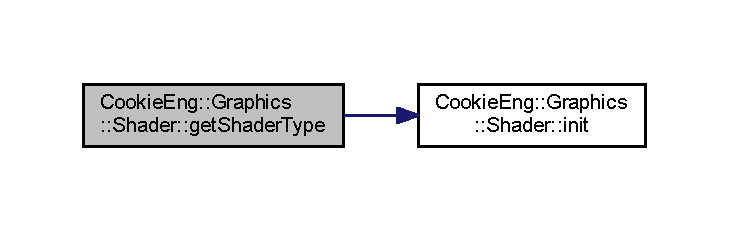
\includegraphics[width=350pt]{class_cookie_eng_1_1_graphics_1_1_shader_adde0294c86137d22a247bd011b8e40c8_cgraph}
\end{center}
\end{figure}
\mbox{\label{class_cookie_eng_1_1_graphics_1_1_shader_ae591a7107e04f835f1f8dbc42e0035c6}} 
\index{Cookie\+Eng\+::\+Graphics\+::\+Shader@{Cookie\+Eng\+::\+Graphics\+::\+Shader}!init@{init}}
\index{init@{init}!Cookie\+Eng\+::\+Graphics\+::\+Shader@{Cookie\+Eng\+::\+Graphics\+::\+Shader}}
\subsubsection{init()}
{\footnotesize\ttfamily void Cookie\+Eng\+::\+Graphics\+::\+Shader\+::init (\begin{DoxyParamCaption}{ }\end{DoxyParamCaption})\hspace{0.3cm}{\ttfamily [protected]}}



Initialises the \doxyref{Shader}{p.}{class_cookie_eng_1_1_graphics_1_1_shader}. 

Creates the shader on the G\+PU. This is seperated from the Constructor as initialising there was causing issues. \mbox{\label{class_cookie_eng_1_1_graphics_1_1_shader_aa11548ffaa72d77521576044a122af43}} 
\index{Cookie\+Eng\+::\+Graphics\+::\+Shader@{Cookie\+Eng\+::\+Graphics\+::\+Shader}!load@{load}}
\index{load@{load}!Cookie\+Eng\+::\+Graphics\+::\+Shader@{Cookie\+Eng\+::\+Graphics\+::\+Shader}}
\subsubsection{load()}
{\footnotesize\ttfamily bool Cookie\+Eng\+::\+Graphics\+::\+Shader\+::load (\begin{DoxyParamCaption}\item[{std\+::string}]{\+\_\+filepath }\end{DoxyParamCaption})}



Loads a text file into the \doxyref{Shader}{p.}{class_cookie_eng_1_1_graphics_1_1_shader}. 


\begin{DoxyParams}{Parameters}
{\em \+\_\+filepath} & The path to the Text File to be loaded \\
\hline
\end{DoxyParams}
\begin{DoxyReturn}{Returns}
the result of the load. True for sucessful, false for error.
\end{DoxyReturn}
Uses the file manager service to load a text file and places it onto the G\+PU. The shader is then verified to ensure the shader source is valid. \mbox{\label{class_cookie_eng_1_1_graphics_1_1_shader_a28abd2dba4a183cb810b196af2e1d5a3}} 
\index{Cookie\+Eng\+::\+Graphics\+::\+Shader@{Cookie\+Eng\+::\+Graphics\+::\+Shader}!verify@{verify}}
\index{verify@{verify}!Cookie\+Eng\+::\+Graphics\+::\+Shader@{Cookie\+Eng\+::\+Graphics\+::\+Shader}}
\subsubsection{verify()}
{\footnotesize\ttfamily bool Cookie\+Eng\+::\+Graphics\+::\+Shader\+::verify (\begin{DoxyParamCaption}{ }\end{DoxyParamCaption})}



Loads a text file into the \doxyref{Shader}{p.}{class_cookie_eng_1_1_graphics_1_1_shader}. 

\begin{DoxyReturn}{Returns}
The result of the verification. True for sucessful, false for error.
\end{DoxyReturn}
Verifies the shader complination and insures it will run. 

\subsection{Member Data Documentation}
\mbox{\label{class_cookie_eng_1_1_graphics_1_1_shader_a3c2b2bf0f97b9367c3871de99378bbbf}} 
\index{Cookie\+Eng\+::\+Graphics\+::\+Shader@{Cookie\+Eng\+::\+Graphics\+::\+Shader}!m\+\_\+shader\+ID@{m\+\_\+shader\+ID}}
\index{m\+\_\+shader\+ID@{m\+\_\+shader\+ID}!Cookie\+Eng\+::\+Graphics\+::\+Shader@{Cookie\+Eng\+::\+Graphics\+::\+Shader}}
\subsubsection{m\+\_\+shader\+ID}
{\footnotesize\ttfamily G\+Luint Cookie\+Eng\+::\+Graphics\+::\+Shader\+::m\+\_\+shader\+ID\hspace{0.3cm}{\ttfamily [protected]}}

The Open\+GL ID \mbox{\label{class_cookie_eng_1_1_graphics_1_1_shader_a50b512033ec7bd695dcd4daa2d971c22}} 
\index{Cookie\+Eng\+::\+Graphics\+::\+Shader@{Cookie\+Eng\+::\+Graphics\+::\+Shader}!m\+\_\+shader\+Type@{m\+\_\+shader\+Type}}
\index{m\+\_\+shader\+Type@{m\+\_\+shader\+Type}!Cookie\+Eng\+::\+Graphics\+::\+Shader@{Cookie\+Eng\+::\+Graphics\+::\+Shader}}
\subsubsection{m\+\_\+shader\+Type}
{\footnotesize\ttfamily Shader\+Type Cookie\+Eng\+::\+Graphics\+::\+Shader\+::m\+\_\+shader\+Type\hspace{0.3cm}{\ttfamily [protected]}}

The \doxyref{Shader}{p.}{class_cookie_eng_1_1_graphics_1_1_shader} Type \mbox{\label{class_cookie_eng_1_1_graphics_1_1_shader_acfa364395f90fdea34e5365221b3b564}} 
\index{Cookie\+Eng\+::\+Graphics\+::\+Shader@{Cookie\+Eng\+::\+Graphics\+::\+Shader}!m\+\_\+verified@{m\+\_\+verified}}
\index{m\+\_\+verified@{m\+\_\+verified}!Cookie\+Eng\+::\+Graphics\+::\+Shader@{Cookie\+Eng\+::\+Graphics\+::\+Shader}}
\subsubsection{m\+\_\+verified}
{\footnotesize\ttfamily bool Cookie\+Eng\+::\+Graphics\+::\+Shader\+::m\+\_\+verified\hspace{0.3cm}{\ttfamily [protected]}}

Flag to indiciate the verification state of the shader 

The documentation for this class was generated from the following file\+:\begin{DoxyCompactItemize}
\item 
include/Shader.\+h\end{DoxyCompactItemize}

\hypertarget{class_cookie_eng_1_1_graphics_1_1_vertex_array}{}\section{Cookie\+Eng\+:\+:Graphics\+:\+:Vertex\+Array Class Reference}
\label{class_cookie_eng_1_1_graphics_1_1_vertex_array}\index{Cookie\+Eng\+::\+Graphics\+::\+Vertex\+Array@{Cookie\+Eng\+::\+Graphics\+::\+Vertex\+Array}}


Absraction of an Open\+GL Vertex Array Object (V\+AO)  




{\ttfamily \#include $<$Vertex\+Array.\+h$>$}

\subsection*{Public Member Functions}
\begin{DoxyCompactItemize}
\item 
\hyperlink{class_cookie_eng_1_1_graphics_1_1_vertex_array_a9ca1229bf83878acd80e947487b2a9ac}{Vertex\+Array} ()
\begin{DoxyCompactList}\small\item\em \hyperlink{class_cookie_eng_1_1_graphics_1_1_vertex_array}{Vertex\+Array} Ctor. \end{DoxyCompactList}\item 
\hyperlink{class_cookie_eng_1_1_graphics_1_1_vertex_array_a114da6690772eaa07108e2dccaa8e93d}{$\sim$\+Vertex\+Array} ()
\begin{DoxyCompactList}\small\item\em \hyperlink{class_cookie_eng_1_1_graphics_1_1_vertex_array}{Vertex\+Array} Dtor. \end{DoxyCompactList}\item 
void \hyperlink{class_cookie_eng_1_1_graphics_1_1_vertex_array_aacb98fcc69be4c0ca1a4d8deb38b053e}{add\+Buffer} (const \hyperlink{class_cookie_eng_1_1_graphics_1_1_vertex_buffer}{Vertex\+Buffer} \&\+\_\+vertex\+Buffer, const \hyperlink{class_cookie_eng_1_1_graphics_1_1_vertex_buffer_layout}{Vertex\+Buffer\+Layout} \&\+\_\+layout)
\begin{DoxyCompactList}\small\item\em Adds a buffer to the V\+AO. \end{DoxyCompactList}\item 
void \hyperlink{class_cookie_eng_1_1_graphics_1_1_vertex_array_afaa952a05a501cb487831cb6e9e052bf}{bind} () const
\begin{DoxyCompactList}\small\item\em \hyperlink{class_cookie_eng_1_1_graphics_1_1_vertex_array}{Vertex\+Array} Dtor. \end{DoxyCompactList}\item 
void \hyperlink{class_cookie_eng_1_1_graphics_1_1_vertex_array_acd3511d77ec22d63984e365e05ef9bcb}{un\+Bind} () const
\begin{DoxyCompactList}\small\item\em \hyperlink{class_cookie_eng_1_1_graphics_1_1_vertex_array}{Vertex\+Array} Dtor. \end{DoxyCompactList}\end{DoxyCompactItemize}
\subsection*{Protected Attributes}
\begin{DoxyCompactItemize}
\item 
G\+Luint \hyperlink{class_cookie_eng_1_1_graphics_1_1_vertex_array_ad4ee57cc45e85deb47a9f2e6a91211a9}{m\+\_\+vertex\+Array\+ID}
\end{DoxyCompactItemize}


\subsection{Detailed Description}
Absraction of an Open\+GL Vertex Array Object (V\+AO) 

This class handles the creation and managment of V\+A\+Os in Open\+GL. It works by assigning Vertex Buffers with a corresponding layout to an array attribute. 

\subsection{Constructor \& Destructor Documentation}
\mbox{\Hypertarget{class_cookie_eng_1_1_graphics_1_1_vertex_array_a9ca1229bf83878acd80e947487b2a9ac}\label{class_cookie_eng_1_1_graphics_1_1_vertex_array_a9ca1229bf83878acd80e947487b2a9ac}} 
\index{Cookie\+Eng\+::\+Graphics\+::\+Vertex\+Array@{Cookie\+Eng\+::\+Graphics\+::\+Vertex\+Array}!Vertex\+Array@{Vertex\+Array}}
\index{Vertex\+Array@{Vertex\+Array}!Cookie\+Eng\+::\+Graphics\+::\+Vertex\+Array@{Cookie\+Eng\+::\+Graphics\+::\+Vertex\+Array}}
\subsubsection{\texorpdfstring{Vertex\+Array()}{VertexArray()}}
{\footnotesize\ttfamily Cookie\+Eng\+::\+Graphics\+::\+Vertex\+Array\+::\+Vertex\+Array (\begin{DoxyParamCaption}{ }\end{DoxyParamCaption})}



\hyperlink{class_cookie_eng_1_1_graphics_1_1_vertex_array}{Vertex\+Array} Ctor. 

Generates a Vertex Array and stores the ID in m\+\_\+vertex\+Array\+ID. \mbox{\Hypertarget{class_cookie_eng_1_1_graphics_1_1_vertex_array_a114da6690772eaa07108e2dccaa8e93d}\label{class_cookie_eng_1_1_graphics_1_1_vertex_array_a114da6690772eaa07108e2dccaa8e93d}} 
\index{Cookie\+Eng\+::\+Graphics\+::\+Vertex\+Array@{Cookie\+Eng\+::\+Graphics\+::\+Vertex\+Array}!````~Vertex\+Array@{$\sim$\+Vertex\+Array}}
\index{````~Vertex\+Array@{$\sim$\+Vertex\+Array}!Cookie\+Eng\+::\+Graphics\+::\+Vertex\+Array@{Cookie\+Eng\+::\+Graphics\+::\+Vertex\+Array}}
\subsubsection{\texorpdfstring{$\sim$\+Vertex\+Array()}{~VertexArray()}}
{\footnotesize\ttfamily Cookie\+Eng\+::\+Graphics\+::\+Vertex\+Array\+::$\sim$\+Vertex\+Array (\begin{DoxyParamCaption}{ }\end{DoxyParamCaption})}



\hyperlink{class_cookie_eng_1_1_graphics_1_1_vertex_array}{Vertex\+Array} Dtor. 

Deletes the Vertex Array 

\subsection{Member Function Documentation}
\mbox{\Hypertarget{class_cookie_eng_1_1_graphics_1_1_vertex_array_aacb98fcc69be4c0ca1a4d8deb38b053e}\label{class_cookie_eng_1_1_graphics_1_1_vertex_array_aacb98fcc69be4c0ca1a4d8deb38b053e}} 
\index{Cookie\+Eng\+::\+Graphics\+::\+Vertex\+Array@{Cookie\+Eng\+::\+Graphics\+::\+Vertex\+Array}!add\+Buffer@{add\+Buffer}}
\index{add\+Buffer@{add\+Buffer}!Cookie\+Eng\+::\+Graphics\+::\+Vertex\+Array@{Cookie\+Eng\+::\+Graphics\+::\+Vertex\+Array}}
\subsubsection{\texorpdfstring{add\+Buffer()}{addBuffer()}}
{\footnotesize\ttfamily void Cookie\+Eng\+::\+Graphics\+::\+Vertex\+Array\+::add\+Buffer (\begin{DoxyParamCaption}\item[{const \hyperlink{class_cookie_eng_1_1_graphics_1_1_vertex_buffer}{Vertex\+Buffer} \&}]{\+\_\+vertex\+Buffer,  }\item[{const \hyperlink{class_cookie_eng_1_1_graphics_1_1_vertex_buffer_layout}{Vertex\+Buffer\+Layout} \&}]{\+\_\+layout }\end{DoxyParamCaption})}



Adds a buffer to the V\+AO. 


\begin{DoxyParams}{Parameters}
{\em \+\_\+vertex\+Buffer} & The vertex buffer to be added to the array. \\
\hline
{\em \+\_\+layout} & The layout of the corresponding buffer.\\
\hline
\end{DoxyParams}
Takes a V\+BO, binds it to the V\+AO and sets up the gl\+Vertex\+Attrib\+Pointer based on the layout provided. \mbox{\Hypertarget{class_cookie_eng_1_1_graphics_1_1_vertex_array_afaa952a05a501cb487831cb6e9e052bf}\label{class_cookie_eng_1_1_graphics_1_1_vertex_array_afaa952a05a501cb487831cb6e9e052bf}} 
\index{Cookie\+Eng\+::\+Graphics\+::\+Vertex\+Array@{Cookie\+Eng\+::\+Graphics\+::\+Vertex\+Array}!bind@{bind}}
\index{bind@{bind}!Cookie\+Eng\+::\+Graphics\+::\+Vertex\+Array@{Cookie\+Eng\+::\+Graphics\+::\+Vertex\+Array}}
\subsubsection{\texorpdfstring{bind()}{bind()}}
{\footnotesize\ttfamily void Cookie\+Eng\+::\+Graphics\+::\+Vertex\+Array\+::bind (\begin{DoxyParamCaption}{ }\end{DoxyParamCaption}) const\hspace{0.3cm}{\ttfamily [inline]}}



\hyperlink{class_cookie_eng_1_1_graphics_1_1_vertex_array}{Vertex\+Array} Dtor. 

Binds the Vertex Array Object (V\+AO) \mbox{\Hypertarget{class_cookie_eng_1_1_graphics_1_1_vertex_array_acd3511d77ec22d63984e365e05ef9bcb}\label{class_cookie_eng_1_1_graphics_1_1_vertex_array_acd3511d77ec22d63984e365e05ef9bcb}} 
\index{Cookie\+Eng\+::\+Graphics\+::\+Vertex\+Array@{Cookie\+Eng\+::\+Graphics\+::\+Vertex\+Array}!un\+Bind@{un\+Bind}}
\index{un\+Bind@{un\+Bind}!Cookie\+Eng\+::\+Graphics\+::\+Vertex\+Array@{Cookie\+Eng\+::\+Graphics\+::\+Vertex\+Array}}
\subsubsection{\texorpdfstring{un\+Bind()}{unBind()}}
{\footnotesize\ttfamily void Cookie\+Eng\+::\+Graphics\+::\+Vertex\+Array\+::un\+Bind (\begin{DoxyParamCaption}{ }\end{DoxyParamCaption}) const\hspace{0.3cm}{\ttfamily [inline]}}



\hyperlink{class_cookie_eng_1_1_graphics_1_1_vertex_array}{Vertex\+Array} Dtor. 

Unbinds the Vertex Array Object (V\+AO) 

\subsection{Member Data Documentation}
\mbox{\Hypertarget{class_cookie_eng_1_1_graphics_1_1_vertex_array_ad4ee57cc45e85deb47a9f2e6a91211a9}\label{class_cookie_eng_1_1_graphics_1_1_vertex_array_ad4ee57cc45e85deb47a9f2e6a91211a9}} 
\index{Cookie\+Eng\+::\+Graphics\+::\+Vertex\+Array@{Cookie\+Eng\+::\+Graphics\+::\+Vertex\+Array}!m\+\_\+vertex\+Array\+ID@{m\+\_\+vertex\+Array\+ID}}
\index{m\+\_\+vertex\+Array\+ID@{m\+\_\+vertex\+Array\+ID}!Cookie\+Eng\+::\+Graphics\+::\+Vertex\+Array@{Cookie\+Eng\+::\+Graphics\+::\+Vertex\+Array}}
\subsubsection{\texorpdfstring{m\+\_\+vertex\+Array\+ID}{m\_vertexArrayID}}
{\footnotesize\ttfamily G\+Luint Cookie\+Eng\+::\+Graphics\+::\+Vertex\+Array\+::m\+\_\+vertex\+Array\+ID\hspace{0.3cm}{\ttfamily [protected]}}

The Open\+GL ID of the V\+AO 

The documentation for this class was generated from the following file\+:\begin{DoxyCompactItemize}
\item 
D\+:/\+Programming/\+Engine Development/\+Cookie\+Eng/\+Cookie\+Eng/include/Vertex\+Array.\+h\end{DoxyCompactItemize}

\hypertarget{class_cookie_eng_1_1_graphics_1_1_vertex_buffer}{}\section{Cookie\+Eng\+:\+:Graphics\+:\+:Vertex\+Buffer Class Reference}
\label{class_cookie_eng_1_1_graphics_1_1_vertex_buffer}\index{Cookie\+Eng\+::\+Graphics\+::\+Vertex\+Buffer@{Cookie\+Eng\+::\+Graphics\+::\+Vertex\+Buffer}}


An abstraction of an Open\+GL Vertex Bufer Object (V\+BO).  




{\ttfamily \#include $<$Vertex\+Buffer.\+h$>$}

\subsection*{Public Member Functions}
\begin{DoxyCompactItemize}
\item 
\hyperlink{class_cookie_eng_1_1_graphics_1_1_vertex_buffer_ac877c409fdb8a09947bb13664b78a335}{Vertex\+Buffer} (const Vertex\+Buffer\+Type \+\_\+type)
\begin{DoxyCompactList}\small\item\em Vertex Buffer Ctor. \end{DoxyCompactList}\item 
\hyperlink{class_cookie_eng_1_1_graphics_1_1_vertex_buffer_af4ceb32a35ff5747f2f80c8cec1e7800}{Vertex\+Buffer} (const Vertex\+Buffer\+Type \+\_\+type, const void $\ast$\+\_\+data, G\+Luint \+\_\+count, G\+Luint \+\_\+size)
\begin{DoxyCompactList}\small\item\em Vertex Buffer Ctor. \end{DoxyCompactList}\item 
\hyperlink{class_cookie_eng_1_1_graphics_1_1_vertex_buffer_a7c664866737550113380e8f08feca778}{$\sim$\+Vertex\+Buffer} ()
\begin{DoxyCompactList}\small\item\em Vertex Buffer Dtor. \end{DoxyCompactList}\item 
\mbox{\Hypertarget{class_cookie_eng_1_1_graphics_1_1_vertex_buffer_a67b3089f2822a48fe31c84e94d087d68}\label{class_cookie_eng_1_1_graphics_1_1_vertex_buffer_a67b3089f2822a48fe31c84e94d087d68}} 
void \hyperlink{class_cookie_eng_1_1_graphics_1_1_vertex_buffer_a67b3089f2822a48fe31c84e94d087d68}{init} ()
\begin{DoxyCompactList}\small\item\em Generates the V\+BO. This is done through this method to avoid issues of using Open\+GL calls in constructors. \end{DoxyCompactList}\item 
void \hyperlink{class_cookie_eng_1_1_graphics_1_1_vertex_buffer_ac3db6a2571101d1836fab492971c75fa}{load\+Data} (const void $\ast$\+\_\+data, G\+Luint \+\_\+count, G\+Luint \+\_\+size)
\begin{DoxyCompactList}\small\item\em Loads data to the V\+BO. \end{DoxyCompactList}\item 
G\+Luint \hyperlink{class_cookie_eng_1_1_graphics_1_1_vertex_buffer_a667b81c15525bd5f76d979e0c8b02be0}{get\+Count} () const
\begin{DoxyCompactList}\small\item\em Returns the count of the number of items contained within the buffer. \end{DoxyCompactList}\item 
void \hyperlink{class_cookie_eng_1_1_graphics_1_1_vertex_buffer_a6fbaa64c5edeb00d4f5770587eb7b369}{bind} () const
\begin{DoxyCompactList}\small\item\em Binds the V\+BO. \end{DoxyCompactList}\item 
void \hyperlink{class_cookie_eng_1_1_graphics_1_1_vertex_buffer_a8fbc3f39762c511438bc13e8c405926c}{un\+Bind} () const
\begin{DoxyCompactList}\small\item\em Unbinds the V\+BO. \end{DoxyCompactList}\item 
void \hyperlink{class_cookie_eng_1_1_graphics_1_1_vertex_buffer_a3098cec29d253dd295586fc92bc48001}{bind\+Base} (G\+Luint \+\_\+index)
\begin{DoxyCompactList}\small\item\em Bind the buffer to an indexed buffer target. \end{DoxyCompactList}\end{DoxyCompactItemize}
\subsection*{Protected Attributes}
\begin{DoxyCompactItemize}
\item 
Vertex\+Buffer\+Type \hyperlink{class_cookie_eng_1_1_graphics_1_1_vertex_buffer_a37d75d306f50db1b63c22b51912402cc}{m\+\_\+vertex\+Buffer\+Type}
\item 
G\+Luint \hyperlink{class_cookie_eng_1_1_graphics_1_1_vertex_buffer_a280a08a319717cf425435efd9b912ef3}{m\+\_\+count}
\item 
G\+Luint \hyperlink{class_cookie_eng_1_1_graphics_1_1_vertex_buffer_af4c00fbd9352dd8a0b5952c007037e2e}{m\+\_\+vertex\+Buffer\+ID}
\end{DoxyCompactItemize}


\subsection{Detailed Description}
An abstraction of an Open\+GL Vertex Bufer Object (V\+BO). 

An anstraction of the Open\+GL Vertex Buffer Object (V\+BO). This is used by the \hyperlink{class_cookie_eng_1_1_graphics_1_1_vertex_array}{Vertex\+Array} class along with a \hyperlink{class_cookie_eng_1_1_graphics_1_1_vertex_buffer_layout}{Vertex\+Buffer\+Layout} for drawing objects. 

\subsection{Constructor \& Destructor Documentation}
\mbox{\Hypertarget{class_cookie_eng_1_1_graphics_1_1_vertex_buffer_ac877c409fdb8a09947bb13664b78a335}\label{class_cookie_eng_1_1_graphics_1_1_vertex_buffer_ac877c409fdb8a09947bb13664b78a335}} 
\index{Cookie\+Eng\+::\+Graphics\+::\+Vertex\+Buffer@{Cookie\+Eng\+::\+Graphics\+::\+Vertex\+Buffer}!Vertex\+Buffer@{Vertex\+Buffer}}
\index{Vertex\+Buffer@{Vertex\+Buffer}!Cookie\+Eng\+::\+Graphics\+::\+Vertex\+Buffer@{Cookie\+Eng\+::\+Graphics\+::\+Vertex\+Buffer}}
\subsubsection{\texorpdfstring{Vertex\+Buffer()}{VertexBuffer()}\hspace{0.1cm}{\footnotesize\ttfamily [1/2]}}
{\footnotesize\ttfamily Cookie\+Eng\+::\+Graphics\+::\+Vertex\+Buffer\+::\+Vertex\+Buffer (\begin{DoxyParamCaption}\item[{const Vertex\+Buffer\+Type}]{\+\_\+type }\end{DoxyParamCaption})}



Vertex Buffer Ctor. 


\begin{DoxyParams}{Parameters}
{\em \+\_\+type} & The V\+BO type to create\\
\hline
\end{DoxyParams}
Generates a Vertex Buffer Object (V\+BO) for use by Open\+GL of the specified type. \mbox{\Hypertarget{class_cookie_eng_1_1_graphics_1_1_vertex_buffer_af4ceb32a35ff5747f2f80c8cec1e7800}\label{class_cookie_eng_1_1_graphics_1_1_vertex_buffer_af4ceb32a35ff5747f2f80c8cec1e7800}} 
\index{Cookie\+Eng\+::\+Graphics\+::\+Vertex\+Buffer@{Cookie\+Eng\+::\+Graphics\+::\+Vertex\+Buffer}!Vertex\+Buffer@{Vertex\+Buffer}}
\index{Vertex\+Buffer@{Vertex\+Buffer}!Cookie\+Eng\+::\+Graphics\+::\+Vertex\+Buffer@{Cookie\+Eng\+::\+Graphics\+::\+Vertex\+Buffer}}
\subsubsection{\texorpdfstring{Vertex\+Buffer()}{VertexBuffer()}\hspace{0.1cm}{\footnotesize\ttfamily [2/2]}}
{\footnotesize\ttfamily Cookie\+Eng\+::\+Graphics\+::\+Vertex\+Buffer\+::\+Vertex\+Buffer (\begin{DoxyParamCaption}\item[{const Vertex\+Buffer\+Type}]{\+\_\+type,  }\item[{const void $\ast$}]{\+\_\+data,  }\item[{G\+Luint}]{\+\_\+count,  }\item[{G\+Luint}]{\+\_\+size }\end{DoxyParamCaption})}



Vertex Buffer Ctor. 


\begin{DoxyParams}{Parameters}
{\em \+\_\+type} & The V\+BO type to create \\
\hline
{\em \+\_\+data} & The data to send to the V\+BO \\
\hline
{\em \+\_\+count} & The number of items of data \\
\hline
{\em \+\_\+size} & The size of the data in bytes\\
\hline
\end{DoxyParams}
Generates a Vertex Buffer Object (V\+BO) through the \hyperlink{class_cookie_eng_1_1_graphics_1_1_vertex_buffer_a67b3089f2822a48fe31c84e94d087d68}{init()} method for use by Open\+GL of the specified type. Also sends the specified data to the V\+BO with the size provided. \mbox{\Hypertarget{class_cookie_eng_1_1_graphics_1_1_vertex_buffer_a7c664866737550113380e8f08feca778}\label{class_cookie_eng_1_1_graphics_1_1_vertex_buffer_a7c664866737550113380e8f08feca778}} 
\index{Cookie\+Eng\+::\+Graphics\+::\+Vertex\+Buffer@{Cookie\+Eng\+::\+Graphics\+::\+Vertex\+Buffer}!````~Vertex\+Buffer@{$\sim$\+Vertex\+Buffer}}
\index{````~Vertex\+Buffer@{$\sim$\+Vertex\+Buffer}!Cookie\+Eng\+::\+Graphics\+::\+Vertex\+Buffer@{Cookie\+Eng\+::\+Graphics\+::\+Vertex\+Buffer}}
\subsubsection{\texorpdfstring{$\sim$\+Vertex\+Buffer()}{~VertexBuffer()}}
{\footnotesize\ttfamily Cookie\+Eng\+::\+Graphics\+::\+Vertex\+Buffer\+::$\sim$\+Vertex\+Buffer (\begin{DoxyParamCaption}{ }\end{DoxyParamCaption})}



Vertex Buffer Dtor. 

Deletes the Vertex Buffer 

\subsection{Member Function Documentation}
\mbox{\Hypertarget{class_cookie_eng_1_1_graphics_1_1_vertex_buffer_a6fbaa64c5edeb00d4f5770587eb7b369}\label{class_cookie_eng_1_1_graphics_1_1_vertex_buffer_a6fbaa64c5edeb00d4f5770587eb7b369}} 
\index{Cookie\+Eng\+::\+Graphics\+::\+Vertex\+Buffer@{Cookie\+Eng\+::\+Graphics\+::\+Vertex\+Buffer}!bind@{bind}}
\index{bind@{bind}!Cookie\+Eng\+::\+Graphics\+::\+Vertex\+Buffer@{Cookie\+Eng\+::\+Graphics\+::\+Vertex\+Buffer}}
\subsubsection{\texorpdfstring{bind()}{bind()}}
{\footnotesize\ttfamily void Cookie\+Eng\+::\+Graphics\+::\+Vertex\+Buffer\+::bind (\begin{DoxyParamCaption}{ }\end{DoxyParamCaption}) const}



Binds the V\+BO. 

Binds the V\+BO. \mbox{\Hypertarget{class_cookie_eng_1_1_graphics_1_1_vertex_buffer_a3098cec29d253dd295586fc92bc48001}\label{class_cookie_eng_1_1_graphics_1_1_vertex_buffer_a3098cec29d253dd295586fc92bc48001}} 
\index{Cookie\+Eng\+::\+Graphics\+::\+Vertex\+Buffer@{Cookie\+Eng\+::\+Graphics\+::\+Vertex\+Buffer}!bind\+Base@{bind\+Base}}
\index{bind\+Base@{bind\+Base}!Cookie\+Eng\+::\+Graphics\+::\+Vertex\+Buffer@{Cookie\+Eng\+::\+Graphics\+::\+Vertex\+Buffer}}
\subsubsection{\texorpdfstring{bind\+Base()}{bindBase()}}
{\footnotesize\ttfamily void Cookie\+Eng\+::\+Graphics\+::\+Vertex\+Buffer\+::bind\+Base (\begin{DoxyParamCaption}\item[{G\+Luint}]{\+\_\+index }\end{DoxyParamCaption})}



Bind the buffer to an indexed buffer target. 


\begin{DoxyParams}{Parameters}
{\em \+\_\+index} & The index of the binding point\\
\hline
\end{DoxyParams}
Binds the buffer object buffer to the binding point at index index of the array of targets specified by target. (Copied from Kkronos.\+org) \mbox{\Hypertarget{class_cookie_eng_1_1_graphics_1_1_vertex_buffer_a667b81c15525bd5f76d979e0c8b02be0}\label{class_cookie_eng_1_1_graphics_1_1_vertex_buffer_a667b81c15525bd5f76d979e0c8b02be0}} 
\index{Cookie\+Eng\+::\+Graphics\+::\+Vertex\+Buffer@{Cookie\+Eng\+::\+Graphics\+::\+Vertex\+Buffer}!get\+Count@{get\+Count}}
\index{get\+Count@{get\+Count}!Cookie\+Eng\+::\+Graphics\+::\+Vertex\+Buffer@{Cookie\+Eng\+::\+Graphics\+::\+Vertex\+Buffer}}
\subsubsection{\texorpdfstring{get\+Count()}{getCount()}}
{\footnotesize\ttfamily G\+Luint Cookie\+Eng\+::\+Graphics\+::\+Vertex\+Buffer\+::get\+Count (\begin{DoxyParamCaption}{ }\end{DoxyParamCaption}) const\hspace{0.3cm}{\ttfamily [inline]}}



Returns the count of the number of items contained within the buffer. 

Returns the count of the number of items contained within the buffer. \mbox{\Hypertarget{class_cookie_eng_1_1_graphics_1_1_vertex_buffer_ac3db6a2571101d1836fab492971c75fa}\label{class_cookie_eng_1_1_graphics_1_1_vertex_buffer_ac3db6a2571101d1836fab492971c75fa}} 
\index{Cookie\+Eng\+::\+Graphics\+::\+Vertex\+Buffer@{Cookie\+Eng\+::\+Graphics\+::\+Vertex\+Buffer}!load\+Data@{load\+Data}}
\index{load\+Data@{load\+Data}!Cookie\+Eng\+::\+Graphics\+::\+Vertex\+Buffer@{Cookie\+Eng\+::\+Graphics\+::\+Vertex\+Buffer}}
\subsubsection{\texorpdfstring{load\+Data()}{loadData()}}
{\footnotesize\ttfamily void Cookie\+Eng\+::\+Graphics\+::\+Vertex\+Buffer\+::load\+Data (\begin{DoxyParamCaption}\item[{const void $\ast$}]{\+\_\+data,  }\item[{G\+Luint}]{\+\_\+count,  }\item[{G\+Luint}]{\+\_\+size }\end{DoxyParamCaption})}



Loads data to the V\+BO. 


\begin{DoxyParams}{Parameters}
{\em \+\_\+data} & he data to send to the V\+BO \\
\hline
{\em \+\_\+count} & The number of items of data \\
\hline
{\em \+\_\+size} & The size of the data in bytes\\
\hline
\end{DoxyParams}
Loads data to the V\+BO. \mbox{\Hypertarget{class_cookie_eng_1_1_graphics_1_1_vertex_buffer_a8fbc3f39762c511438bc13e8c405926c}\label{class_cookie_eng_1_1_graphics_1_1_vertex_buffer_a8fbc3f39762c511438bc13e8c405926c}} 
\index{Cookie\+Eng\+::\+Graphics\+::\+Vertex\+Buffer@{Cookie\+Eng\+::\+Graphics\+::\+Vertex\+Buffer}!un\+Bind@{un\+Bind}}
\index{un\+Bind@{un\+Bind}!Cookie\+Eng\+::\+Graphics\+::\+Vertex\+Buffer@{Cookie\+Eng\+::\+Graphics\+::\+Vertex\+Buffer}}
\subsubsection{\texorpdfstring{un\+Bind()}{unBind()}}
{\footnotesize\ttfamily void Cookie\+Eng\+::\+Graphics\+::\+Vertex\+Buffer\+::un\+Bind (\begin{DoxyParamCaption}{ }\end{DoxyParamCaption}) const}



Unbinds the V\+BO. 

Unbinds the V\+BO. 

\subsection{Member Data Documentation}
\mbox{\Hypertarget{class_cookie_eng_1_1_graphics_1_1_vertex_buffer_a280a08a319717cf425435efd9b912ef3}\label{class_cookie_eng_1_1_graphics_1_1_vertex_buffer_a280a08a319717cf425435efd9b912ef3}} 
\index{Cookie\+Eng\+::\+Graphics\+::\+Vertex\+Buffer@{Cookie\+Eng\+::\+Graphics\+::\+Vertex\+Buffer}!m\+\_\+count@{m\+\_\+count}}
\index{m\+\_\+count@{m\+\_\+count}!Cookie\+Eng\+::\+Graphics\+::\+Vertex\+Buffer@{Cookie\+Eng\+::\+Graphics\+::\+Vertex\+Buffer}}
\subsubsection{\texorpdfstring{m\+\_\+count}{m\_count}}
{\footnotesize\ttfamily G\+Luint Cookie\+Eng\+::\+Graphics\+::\+Vertex\+Buffer\+::m\+\_\+count\hspace{0.3cm}{\ttfamily [protected]}}

The number of items of data there is in the buffer \mbox{\Hypertarget{class_cookie_eng_1_1_graphics_1_1_vertex_buffer_af4c00fbd9352dd8a0b5952c007037e2e}\label{class_cookie_eng_1_1_graphics_1_1_vertex_buffer_af4c00fbd9352dd8a0b5952c007037e2e}} 
\index{Cookie\+Eng\+::\+Graphics\+::\+Vertex\+Buffer@{Cookie\+Eng\+::\+Graphics\+::\+Vertex\+Buffer}!m\+\_\+vertex\+Buffer\+ID@{m\+\_\+vertex\+Buffer\+ID}}
\index{m\+\_\+vertex\+Buffer\+ID@{m\+\_\+vertex\+Buffer\+ID}!Cookie\+Eng\+::\+Graphics\+::\+Vertex\+Buffer@{Cookie\+Eng\+::\+Graphics\+::\+Vertex\+Buffer}}
\subsubsection{\texorpdfstring{m\+\_\+vertex\+Buffer\+ID}{m\_vertexBufferID}}
{\footnotesize\ttfamily G\+Luint Cookie\+Eng\+::\+Graphics\+::\+Vertex\+Buffer\+::m\+\_\+vertex\+Buffer\+ID\hspace{0.3cm}{\ttfamily [protected]}}

The Vertex Buffer ID \mbox{\Hypertarget{class_cookie_eng_1_1_graphics_1_1_vertex_buffer_a37d75d306f50db1b63c22b51912402cc}\label{class_cookie_eng_1_1_graphics_1_1_vertex_buffer_a37d75d306f50db1b63c22b51912402cc}} 
\index{Cookie\+Eng\+::\+Graphics\+::\+Vertex\+Buffer@{Cookie\+Eng\+::\+Graphics\+::\+Vertex\+Buffer}!m\+\_\+vertex\+Buffer\+Type@{m\+\_\+vertex\+Buffer\+Type}}
\index{m\+\_\+vertex\+Buffer\+Type@{m\+\_\+vertex\+Buffer\+Type}!Cookie\+Eng\+::\+Graphics\+::\+Vertex\+Buffer@{Cookie\+Eng\+::\+Graphics\+::\+Vertex\+Buffer}}
\subsubsection{\texorpdfstring{m\+\_\+vertex\+Buffer\+Type}{m\_vertexBufferType}}
{\footnotesize\ttfamily Vertex\+Buffer\+Type Cookie\+Eng\+::\+Graphics\+::\+Vertex\+Buffer\+::m\+\_\+vertex\+Buffer\+Type\hspace{0.3cm}{\ttfamily [protected]}}

The type of Vertex Buffer (B\+U\+F\+F\+E\+R\+\_\+\+A\+R\+R\+AY, B\+U\+F\+F\+E\+R\+\_\+\+E\+L\+E\+M\+E\+N\+T\+\_\+\+A\+R\+R\+AY, etc) 

The documentation for this class was generated from the following file\+:\begin{DoxyCompactItemize}
\item 
D\+:/\+Programming/\+Engine Development/\+Cookie\+Eng/\+Cookie\+Eng/include/Vertex\+Buffer.\+h\end{DoxyCompactItemize}

\section{Cookie\+Eng\+:\+:Graphics\+:\+:Vertex\+Buffer\+Element Class Reference}
\label{struct_cookie_eng_1_1_graphics_1_1_vertex_buffer_element}\index{Cookie\+Eng\+::\+Graphics\+::\+Vertex\+Buffer\+Element@{Cookie\+Eng\+::\+Graphics\+::\+Vertex\+Buffer\+Element}}


Represents an element of a layout of data stored in a V\+AO.  




{\ttfamily \#include $<$Vertex\+Buffer\+Layout.\+h$>$}

\subsection*{Static Public Member Functions}
\begin{DoxyCompactItemize}
\item 
static unsigned int \textbf{ get\+Size\+Of\+Type} (unsigned int \+\_\+type)
\begin{DoxyCompactList}\small\item\em Gets the size of a supported element type. \end{DoxyCompactList}\end{DoxyCompactItemize}
\subsection*{Public Attributes}
\begin{DoxyCompactItemize}
\item 
G\+Luint \textbf{ type}
\item 
G\+Luint \textbf{ count}
\item 
unsigned char \textbf{ normalised}
\end{DoxyCompactItemize}


\subsection{Detailed Description}
Represents an element of a layout of data stored in a V\+AO. 

This class is used in the \doxyref{Vertex\+Buffer\+Layout}{p.}{class_cookie_eng_1_1_graphics_1_1_vertex_buffer_layout} class to store an element of a layout 

\subsection{Member Function Documentation}
\mbox{\label{struct_cookie_eng_1_1_graphics_1_1_vertex_buffer_element_a2041f09a7eb0714959f1be6f67fb111b}} 
\index{Cookie\+Eng\+::\+Graphics\+::\+Vertex\+Buffer\+Element@{Cookie\+Eng\+::\+Graphics\+::\+Vertex\+Buffer\+Element}!get\+Size\+Of\+Type@{get\+Size\+Of\+Type}}
\index{get\+Size\+Of\+Type@{get\+Size\+Of\+Type}!Cookie\+Eng\+::\+Graphics\+::\+Vertex\+Buffer\+Element@{Cookie\+Eng\+::\+Graphics\+::\+Vertex\+Buffer\+Element}}
\subsubsection{get\+Size\+Of\+Type()}
{\footnotesize\ttfamily static unsigned int Cookie\+Eng\+::\+Graphics\+::\+Vertex\+Buffer\+Element\+::get\+Size\+Of\+Type (\begin{DoxyParamCaption}\item[{unsigned int}]{\+\_\+type }\end{DoxyParamCaption})\hspace{0.3cm}{\ttfamily [inline]}, {\ttfamily [static]}}



Gets the size of a supported element type. 


\begin{DoxyParams}{Parameters}
{\em \+\_\+type} & The type to return the size of \\
\hline
\end{DoxyParams}
\begin{DoxyReturn}{Returns}
the byte size of the type specified by the parameter
\end{DoxyReturn}
Takes in a data type and returns the size of that type. This method will only return the size of supported data types that can be added to a V\+BO (layout or actual V\+BO). 

\subsection{Member Data Documentation}
\mbox{\label{struct_cookie_eng_1_1_graphics_1_1_vertex_buffer_element_a5c5d5a5861ed76486f0ea36e8db6ed4c}} 
\index{Cookie\+Eng\+::\+Graphics\+::\+Vertex\+Buffer\+Element@{Cookie\+Eng\+::\+Graphics\+::\+Vertex\+Buffer\+Element}!count@{count}}
\index{count@{count}!Cookie\+Eng\+::\+Graphics\+::\+Vertex\+Buffer\+Element@{Cookie\+Eng\+::\+Graphics\+::\+Vertex\+Buffer\+Element}}
\subsubsection{count}
{\footnotesize\ttfamily G\+Luint Cookie\+Eng\+::\+Graphics\+::\+Vertex\+Buffer\+Element\+::count}

The number of the specified type stored in the element (eg, 3 for a vec3 as it is 3 floats) \mbox{\label{struct_cookie_eng_1_1_graphics_1_1_vertex_buffer_element_a1a50c45bd6f7e11f158b142ec20552ba}} 
\index{Cookie\+Eng\+::\+Graphics\+::\+Vertex\+Buffer\+Element@{Cookie\+Eng\+::\+Graphics\+::\+Vertex\+Buffer\+Element}!normalised@{normalised}}
\index{normalised@{normalised}!Cookie\+Eng\+::\+Graphics\+::\+Vertex\+Buffer\+Element@{Cookie\+Eng\+::\+Graphics\+::\+Vertex\+Buffer\+Element}}
\subsubsection{normalised}
{\footnotesize\ttfamily unsigned char Cookie\+Eng\+::\+Graphics\+::\+Vertex\+Buffer\+Element\+::normalised}

Wether the data is normalised (between -\/1.\+0 and 1.\+0) \mbox{\label{struct_cookie_eng_1_1_graphics_1_1_vertex_buffer_element_abba091f340c618809735781f80ccee6b}} 
\index{Cookie\+Eng\+::\+Graphics\+::\+Vertex\+Buffer\+Element@{Cookie\+Eng\+::\+Graphics\+::\+Vertex\+Buffer\+Element}!type@{type}}
\index{type@{type}!Cookie\+Eng\+::\+Graphics\+::\+Vertex\+Buffer\+Element@{Cookie\+Eng\+::\+Graphics\+::\+Vertex\+Buffer\+Element}}
\subsubsection{type}
{\footnotesize\ttfamily G\+Luint Cookie\+Eng\+::\+Graphics\+::\+Vertex\+Buffer\+Element\+::type}

The data type of the element 

The documentation for this class was generated from the following file\+:\begin{DoxyCompactItemize}
\item 
include/Vertex\+Buffer\+Layout.\+h\end{DoxyCompactItemize}

\hypertarget{class_cookie_eng_1_1_graphics_1_1_vertex_buffer_layout}{}\section{Cookie\+Eng\+:\+:Graphics\+:\+:Vertex\+Buffer\+Layout Class Reference}
\label{class_cookie_eng_1_1_graphics_1_1_vertex_buffer_layout}\index{Cookie\+Eng\+::\+Graphics\+::\+Vertex\+Buffer\+Layout@{Cookie\+Eng\+::\+Graphics\+::\+Vertex\+Buffer\+Layout}}


Abstraction of the layout of a V\+BO.  




{\ttfamily \#include $<$Vertex\+Buffer\+Layout.\+h$>$}

\subsection*{Public Member Functions}
\begin{DoxyCompactItemize}
\item 
{\footnotesize template$<$typename T $>$ }\\void \hyperlink{class_cookie_eng_1_1_graphics_1_1_vertex_buffer_layout_a8d9958c85411d75d7f412b2d3f7b566a}{push} (unsigned int \+\_\+count)
\begin{DoxyCompactList}\small\item\em Pushes a new element to the layout of the specified type. \end{DoxyCompactList}\item 
{\footnotesize template$<$$>$ }\\void \hyperlink{class_cookie_eng_1_1_graphics_1_1_vertex_buffer_layout_a3f1a639714762ec45edf48a68995d7bd}{push} (unsigned int \+\_\+count)
\begin{DoxyCompactList}\small\item\em Pushes a new float element to the layout. \end{DoxyCompactList}\item 
{\footnotesize template$<$$>$ }\\void \hyperlink{class_cookie_eng_1_1_graphics_1_1_vertex_buffer_layout_a3f1a639714762ec45edf48a68995d7bd}{push} (unsigned int \+\_\+count)
\begin{DoxyCompactList}\small\item\em Pushes a new G\+Luint element to the layout. \end{DoxyCompactList}\item 
{\footnotesize template$<$$>$ }\\void \hyperlink{class_cookie_eng_1_1_graphics_1_1_vertex_buffer_layout_a3f1a639714762ec45edf48a68995d7bd}{push} (unsigned int \+\_\+count)
\begin{DoxyCompactList}\small\item\em Pushes a new unsigned char element to the layout. \end{DoxyCompactList}\item 
const std\+::vector$<$ \hyperlink{struct_cookie_eng_1_1_graphics_1_1_vertex_buffer_element}{Vertex\+Buffer\+Element} $>$ \hyperlink{class_cookie_eng_1_1_graphics_1_1_vertex_buffer_layout_a082cc08b182cabe19998ae522c0466be}{get\+Elements} () const
\begin{DoxyCompactList}\small\item\em Returns the vector of elements that make up the layout. \end{DoxyCompactList}\item 
G\+Luint \hyperlink{class_cookie_eng_1_1_graphics_1_1_vertex_buffer_layout_a4c771d06898767d1a92237b03a53e887}{get\+Stride} () const
\begin{DoxyCompactList}\small\item\em Returns the stride of the layout. \end{DoxyCompactList}\item 
void \hyperlink{class_cookie_eng_1_1_graphics_1_1_vertex_buffer_layout_a9e511f18b0895825ff8ea2b567f89626}{reset} ()
\begin{DoxyCompactList}\small\item\em Resets the layout. \end{DoxyCompactList}\end{DoxyCompactItemize}
\subsection*{Protected Attributes}
\begin{DoxyCompactItemize}
\item 
std\+::vector$<$ \hyperlink{struct_cookie_eng_1_1_graphics_1_1_vertex_buffer_element}{Vertex\+Buffer\+Element} $>$ \hyperlink{class_cookie_eng_1_1_graphics_1_1_vertex_buffer_layout_a7986bf1ce59d1ffa1dc31613014aa2e7}{m\+\_\+elements}
\item 
G\+Luint \hyperlink{class_cookie_eng_1_1_graphics_1_1_vertex_buffer_layout_a972f0e9224f28b13be7d959449423308}{m\+\_\+stride}
\end{DoxyCompactItemize}


\subsection{Detailed Description}
Abstraction of the layout of a V\+BO. 

This class stores a vector of elements that make up the layout of data stored in a V\+BO. The push function adds a new element of the templated type to the V\+BO layout. 

\subsection{Member Function Documentation}
\mbox{\Hypertarget{class_cookie_eng_1_1_graphics_1_1_vertex_buffer_layout_a082cc08b182cabe19998ae522c0466be}\label{class_cookie_eng_1_1_graphics_1_1_vertex_buffer_layout_a082cc08b182cabe19998ae522c0466be}} 
\index{Cookie\+Eng\+::\+Graphics\+::\+Vertex\+Buffer\+Layout@{Cookie\+Eng\+::\+Graphics\+::\+Vertex\+Buffer\+Layout}!get\+Elements@{get\+Elements}}
\index{get\+Elements@{get\+Elements}!Cookie\+Eng\+::\+Graphics\+::\+Vertex\+Buffer\+Layout@{Cookie\+Eng\+::\+Graphics\+::\+Vertex\+Buffer\+Layout}}
\subsubsection{\texorpdfstring{get\+Elements()}{getElements()}}
{\footnotesize\ttfamily const std\+::vector$<$\hyperlink{struct_cookie_eng_1_1_graphics_1_1_vertex_buffer_element}{Vertex\+Buffer\+Element}$>$ Cookie\+Eng\+::\+Graphics\+::\+Vertex\+Buffer\+Layout\+::get\+Elements (\begin{DoxyParamCaption}{ }\end{DoxyParamCaption}) const\hspace{0.3cm}{\ttfamily [inline]}}



Returns the vector of elements that make up the layout. 

Returns the vector that contains the elements of the layout. These can be read by the V\+AO class and applied to a V\+BO. \mbox{\Hypertarget{class_cookie_eng_1_1_graphics_1_1_vertex_buffer_layout_a4c771d06898767d1a92237b03a53e887}\label{class_cookie_eng_1_1_graphics_1_1_vertex_buffer_layout_a4c771d06898767d1a92237b03a53e887}} 
\index{Cookie\+Eng\+::\+Graphics\+::\+Vertex\+Buffer\+Layout@{Cookie\+Eng\+::\+Graphics\+::\+Vertex\+Buffer\+Layout}!get\+Stride@{get\+Stride}}
\index{get\+Stride@{get\+Stride}!Cookie\+Eng\+::\+Graphics\+::\+Vertex\+Buffer\+Layout@{Cookie\+Eng\+::\+Graphics\+::\+Vertex\+Buffer\+Layout}}
\subsubsection{\texorpdfstring{get\+Stride()}{getStride()}}
{\footnotesize\ttfamily G\+Luint Cookie\+Eng\+::\+Graphics\+::\+Vertex\+Buffer\+Layout\+::get\+Stride (\begin{DoxyParamCaption}{ }\end{DoxyParamCaption}) const\hspace{0.3cm}{\ttfamily [inline]}}



Returns the stride of the layout. 

Returns the stride of the layout (the distance in bytes between one item in the data and the next corresponding item) \mbox{\Hypertarget{class_cookie_eng_1_1_graphics_1_1_vertex_buffer_layout_a8d9958c85411d75d7f412b2d3f7b566a}\label{class_cookie_eng_1_1_graphics_1_1_vertex_buffer_layout_a8d9958c85411d75d7f412b2d3f7b566a}} 
\index{Cookie\+Eng\+::\+Graphics\+::\+Vertex\+Buffer\+Layout@{Cookie\+Eng\+::\+Graphics\+::\+Vertex\+Buffer\+Layout}!push@{push}}
\index{push@{push}!Cookie\+Eng\+::\+Graphics\+::\+Vertex\+Buffer\+Layout@{Cookie\+Eng\+::\+Graphics\+::\+Vertex\+Buffer\+Layout}}
\subsubsection{\texorpdfstring{push()}{push()}\hspace{0.1cm}{\footnotesize\ttfamily [1/4]}}
{\footnotesize\ttfamily template$<$typename T $>$ \\
void Cookie\+Eng\+::\+Graphics\+::\+Vertex\+Buffer\+Layout\+::push (\begin{DoxyParamCaption}\item[{unsigned int}]{\+\_\+count }\end{DoxyParamCaption})\hspace{0.3cm}{\ttfamily [inline]}}



Pushes a new element to the layout of the specified type. 


\begin{DoxyParams}{Parameters}
{\em \+\_\+count} & The number of values in the element. Eg, 3 for a vec3 (3 floats), 2 for a vec2 (2 floats).\\
\hline
\end{DoxyParams}
Pushes a new element into the layout of the templated type and with the specified count (how many items of the specified type make up the element). \mbox{\Hypertarget{class_cookie_eng_1_1_graphics_1_1_vertex_buffer_layout_a3f1a639714762ec45edf48a68995d7bd}\label{class_cookie_eng_1_1_graphics_1_1_vertex_buffer_layout_a3f1a639714762ec45edf48a68995d7bd}} 
\index{Cookie\+Eng\+::\+Graphics\+::\+Vertex\+Buffer\+Layout@{Cookie\+Eng\+::\+Graphics\+::\+Vertex\+Buffer\+Layout}!push@{push}}
\index{push@{push}!Cookie\+Eng\+::\+Graphics\+::\+Vertex\+Buffer\+Layout@{Cookie\+Eng\+::\+Graphics\+::\+Vertex\+Buffer\+Layout}}
\subsubsection{\texorpdfstring{push()}{push()}\hspace{0.1cm}{\footnotesize\ttfamily [2/4]}}
{\footnotesize\ttfamily template$<$$>$ \\
void Cookie\+Eng\+::\+Graphics\+::\+Vertex\+Buffer\+Layout\+::push (\begin{DoxyParamCaption}\item[{unsigned int}]{\+\_\+count }\end{DoxyParamCaption})\hspace{0.3cm}{\ttfamily [inline]}}



Pushes a new float element to the layout. 


\begin{DoxyParams}{Parameters}
{\em \+\_\+count} & The number of values in the element. Eg, 3 for a vec3 (3 floats), 2 for a vec2 (2 floats).\\
\hline
\end{DoxyParams}
Pushes a new float element into the layout with the specified count (how many items of the specified type make up the element). \mbox{\Hypertarget{class_cookie_eng_1_1_graphics_1_1_vertex_buffer_layout_a3f1a639714762ec45edf48a68995d7bd}\label{class_cookie_eng_1_1_graphics_1_1_vertex_buffer_layout_a3f1a639714762ec45edf48a68995d7bd}} 
\index{Cookie\+Eng\+::\+Graphics\+::\+Vertex\+Buffer\+Layout@{Cookie\+Eng\+::\+Graphics\+::\+Vertex\+Buffer\+Layout}!push@{push}}
\index{push@{push}!Cookie\+Eng\+::\+Graphics\+::\+Vertex\+Buffer\+Layout@{Cookie\+Eng\+::\+Graphics\+::\+Vertex\+Buffer\+Layout}}
\subsubsection{\texorpdfstring{push()}{push()}\hspace{0.1cm}{\footnotesize\ttfamily [3/4]}}
{\footnotesize\ttfamily template$<$$>$ \\
void Cookie\+Eng\+::\+Graphics\+::\+Vertex\+Buffer\+Layout\+::push (\begin{DoxyParamCaption}\item[{unsigned int}]{\+\_\+count }\end{DoxyParamCaption})\hspace{0.3cm}{\ttfamily [inline]}}



Pushes a new G\+Luint element to the layout. 


\begin{DoxyParams}{Parameters}
{\em \+\_\+count} & The number of values in the element. Eg, 3 for a vec3 (3 floats), 2 for a vec2 (2 floats).\\
\hline
\end{DoxyParams}
Pushes a new G\+Luint element into the layout with the specified count (how many items of the specified type make up the element). \mbox{\Hypertarget{class_cookie_eng_1_1_graphics_1_1_vertex_buffer_layout_a3f1a639714762ec45edf48a68995d7bd}\label{class_cookie_eng_1_1_graphics_1_1_vertex_buffer_layout_a3f1a639714762ec45edf48a68995d7bd}} 
\index{Cookie\+Eng\+::\+Graphics\+::\+Vertex\+Buffer\+Layout@{Cookie\+Eng\+::\+Graphics\+::\+Vertex\+Buffer\+Layout}!push@{push}}
\index{push@{push}!Cookie\+Eng\+::\+Graphics\+::\+Vertex\+Buffer\+Layout@{Cookie\+Eng\+::\+Graphics\+::\+Vertex\+Buffer\+Layout}}
\subsubsection{\texorpdfstring{push()}{push()}\hspace{0.1cm}{\footnotesize\ttfamily [4/4]}}
{\footnotesize\ttfamily template$<$$>$ \\
void Cookie\+Eng\+::\+Graphics\+::\+Vertex\+Buffer\+Layout\+::push (\begin{DoxyParamCaption}\item[{unsigned int}]{\+\_\+count }\end{DoxyParamCaption})\hspace{0.3cm}{\ttfamily [inline]}}



Pushes a new unsigned char element to the layout. 


\begin{DoxyParams}{Parameters}
{\em \+\_\+count} & The number of values in the element. Eg, 3 for a vec3 (3 floats), 2 for a vec2 (2 floats).\\
\hline
\end{DoxyParams}
Pushes a new unsigned char element into the layout with the specified count (how many items of the specified type make up the element). \mbox{\Hypertarget{class_cookie_eng_1_1_graphics_1_1_vertex_buffer_layout_a9e511f18b0895825ff8ea2b567f89626}\label{class_cookie_eng_1_1_graphics_1_1_vertex_buffer_layout_a9e511f18b0895825ff8ea2b567f89626}} 
\index{Cookie\+Eng\+::\+Graphics\+::\+Vertex\+Buffer\+Layout@{Cookie\+Eng\+::\+Graphics\+::\+Vertex\+Buffer\+Layout}!reset@{reset}}
\index{reset@{reset}!Cookie\+Eng\+::\+Graphics\+::\+Vertex\+Buffer\+Layout@{Cookie\+Eng\+::\+Graphics\+::\+Vertex\+Buffer\+Layout}}
\subsubsection{\texorpdfstring{reset()}{reset()}}
{\footnotesize\ttfamily void Cookie\+Eng\+::\+Graphics\+::\+Vertex\+Buffer\+Layout\+::reset (\begin{DoxyParamCaption}{ }\end{DoxyParamCaption})\hspace{0.3cm}{\ttfamily [inline]}}



Resets the layout. 

Resets the layout back to default 

\subsection{Member Data Documentation}
\mbox{\Hypertarget{class_cookie_eng_1_1_graphics_1_1_vertex_buffer_layout_a7986bf1ce59d1ffa1dc31613014aa2e7}\label{class_cookie_eng_1_1_graphics_1_1_vertex_buffer_layout_a7986bf1ce59d1ffa1dc31613014aa2e7}} 
\index{Cookie\+Eng\+::\+Graphics\+::\+Vertex\+Buffer\+Layout@{Cookie\+Eng\+::\+Graphics\+::\+Vertex\+Buffer\+Layout}!m\+\_\+elements@{m\+\_\+elements}}
\index{m\+\_\+elements@{m\+\_\+elements}!Cookie\+Eng\+::\+Graphics\+::\+Vertex\+Buffer\+Layout@{Cookie\+Eng\+::\+Graphics\+::\+Vertex\+Buffer\+Layout}}
\subsubsection{\texorpdfstring{m\+\_\+elements}{m\_elements}}
{\footnotesize\ttfamily std\+::vector$<$\hyperlink{struct_cookie_eng_1_1_graphics_1_1_vertex_buffer_element}{Vertex\+Buffer\+Element}$>$ Cookie\+Eng\+::\+Graphics\+::\+Vertex\+Buffer\+Layout\+::m\+\_\+elements\hspace{0.3cm}{\ttfamily [protected]}}

The vector containing the elements that make up the layout \mbox{\Hypertarget{class_cookie_eng_1_1_graphics_1_1_vertex_buffer_layout_a972f0e9224f28b13be7d959449423308}\label{class_cookie_eng_1_1_graphics_1_1_vertex_buffer_layout_a972f0e9224f28b13be7d959449423308}} 
\index{Cookie\+Eng\+::\+Graphics\+::\+Vertex\+Buffer\+Layout@{Cookie\+Eng\+::\+Graphics\+::\+Vertex\+Buffer\+Layout}!m\+\_\+stride@{m\+\_\+stride}}
\index{m\+\_\+stride@{m\+\_\+stride}!Cookie\+Eng\+::\+Graphics\+::\+Vertex\+Buffer\+Layout@{Cookie\+Eng\+::\+Graphics\+::\+Vertex\+Buffer\+Layout}}
\subsubsection{\texorpdfstring{m\+\_\+stride}{m\_stride}}
{\footnotesize\ttfamily G\+Luint Cookie\+Eng\+::\+Graphics\+::\+Vertex\+Buffer\+Layout\+::m\+\_\+stride\hspace{0.3cm}{\ttfamily [protected]}}

The stride between data in the layout 

The documentation for this class was generated from the following file\+:\begin{DoxyCompactItemize}
\item 
D\+:/\+Programming/\+Engine Development/\+Cookie\+Eng/\+Cookie\+Eng/include/Vertex\+Buffer\+Layout.\+h\end{DoxyCompactItemize}

\section{Cookie\+Eng\+:\+:Window Class Reference}
\label{class_cookie_eng_1_1_window}\index{Cookie\+Eng\+::\+Window@{Cookie\+Eng\+::\+Window}}


An abstraction of the S\+DL \doxyref{Window}{p.}{class_cookie_eng_1_1_window} class which can be used to create a window for Open\+GL rendering.  




{\ttfamily \#include $<$Window.\+h$>$}

\subsection*{Public Member Functions}
\begin{DoxyCompactItemize}
\item 
\textbf{ Window} (const std\+::string \+\_\+title=\char`\"{}Default\char`\"{}, const int \+\_\+width=1280, const int \+\_\+height=720)
\begin{DoxyCompactList}\small\item\em The \doxyref{Window}{p.}{class_cookie_eng_1_1_window} Constructor. \end{DoxyCompactList}\item 
\textbf{ $\sim$\+Window} ()
\begin{DoxyCompactList}\small\item\em The \doxyref{Window}{p.}{class_cookie_eng_1_1_window} Destructor. \end{DoxyCompactList}\item 
void \textbf{ swap\+Buffer} ()
\begin{DoxyCompactList}\small\item\em \doxyref{Window}{p.}{class_cookie_eng_1_1_window} Buffer Swap. \end{DoxyCompactList}\end{DoxyCompactItemize}
\subsection*{Protected Attributes}
\begin{DoxyCompactItemize}
\item 
S\+D\+L\+\_\+\+Window $\ast$ \textbf{ m\+\_\+window}
\item 
S\+D\+L\+\_\+\+Renderer $\ast$ \textbf{ m\+\_\+renderer}
\item 
S\+D\+L\+\_\+\+G\+L\+Context \textbf{ m\+\_\+open\+G\+L\+Context}
\end{DoxyCompactItemize}


\subsection{Detailed Description}
An abstraction of the S\+DL \doxyref{Window}{p.}{class_cookie_eng_1_1_window} class which can be used to create a window for Open\+GL rendering. 

This class uses the S\+DL \doxyref{Window}{p.}{class_cookie_eng_1_1_window} class to create a window in the constructor. By use of default parameters, a default window can be created by passing no arguments to the constructor or various settings can be applied. An Open\+GL Context is created with the window for rendering. 

\subsection{Constructor \& Destructor Documentation}
\mbox{\label{class_cookie_eng_1_1_window_ada0459ccc0ba0254bb9517cce1cf94bb}} 
\index{Cookie\+Eng\+::\+Window@{Cookie\+Eng\+::\+Window}!Window@{Window}}
\index{Window@{Window}!Cookie\+Eng\+::\+Window@{Cookie\+Eng\+::\+Window}}
\subsubsection{Window()}
{\footnotesize\ttfamily Cookie\+Eng\+::\+Window\+::\+Window (\begin{DoxyParamCaption}\item[{const std\+::string}]{\+\_\+title = {\ttfamily \char`\"{}Default\char`\"{}},  }\item[{const int}]{\+\_\+width = {\ttfamily 1280},  }\item[{const int}]{\+\_\+height = {\ttfamily 720} }\end{DoxyParamCaption})}



The \doxyref{Window}{p.}{class_cookie_eng_1_1_window} Constructor. 


\begin{DoxyParams}{Parameters}
{\em \+\_\+title} & The \doxyref{Window}{p.}{class_cookie_eng_1_1_window} Title that will be displayed in the OS \\
\hline
{\em \+\_\+width} & The default width of the window \\
\hline
{\em \+\_\+height} & The default height of the window\\
\hline
\end{DoxyParams}
The constructor takes default arguments for a standard window but title, width and height can be set by overwriting these provided values. The constructor creates an S\+DL \doxyref{Window}{p.}{class_cookie_eng_1_1_window}, S\+DL Renderer and an accompanying GL Context. \mbox{\label{class_cookie_eng_1_1_window_af81149525fe716874b5637cbef63c78f}} 
\index{Cookie\+Eng\+::\+Window@{Cookie\+Eng\+::\+Window}!````~Window@{$\sim$\+Window}}
\index{````~Window@{$\sim$\+Window}!Cookie\+Eng\+::\+Window@{Cookie\+Eng\+::\+Window}}
\subsubsection{$\sim$\+Window()}
{\footnotesize\ttfamily Cookie\+Eng\+::\+Window\+::$\sim$\+Window (\begin{DoxyParamCaption}{ }\end{DoxyParamCaption})}



The \doxyref{Window}{p.}{class_cookie_eng_1_1_window} Destructor. 

This Destructor simply destorys the S\+DL \doxyref{Window}{p.}{class_cookie_eng_1_1_window} and Renderer. 

\subsection{Member Function Documentation}
\mbox{\label{class_cookie_eng_1_1_window_aebe5875df57a0ab57f3cc9da256dd439}} 
\index{Cookie\+Eng\+::\+Window@{Cookie\+Eng\+::\+Window}!swap\+Buffer@{swap\+Buffer}}
\index{swap\+Buffer@{swap\+Buffer}!Cookie\+Eng\+::\+Window@{Cookie\+Eng\+::\+Window}}
\subsubsection{swap\+Buffer()}
{\footnotesize\ttfamily void Cookie\+Eng\+::\+Window\+::swap\+Buffer (\begin{DoxyParamCaption}{ }\end{DoxyParamCaption})}



\doxyref{Window}{p.}{class_cookie_eng_1_1_window} Buffer Swap. 

This method simply swaps the window buffer. Should be called per frame. 

\subsection{Member Data Documentation}
\mbox{\label{class_cookie_eng_1_1_window_aa4fb697e5f3fb9890da293c6c19d2db4}} 
\index{Cookie\+Eng\+::\+Window@{Cookie\+Eng\+::\+Window}!m\+\_\+open\+G\+L\+Context@{m\+\_\+open\+G\+L\+Context}}
\index{m\+\_\+open\+G\+L\+Context@{m\+\_\+open\+G\+L\+Context}!Cookie\+Eng\+::\+Window@{Cookie\+Eng\+::\+Window}}
\subsubsection{m\+\_\+open\+G\+L\+Context}
{\footnotesize\ttfamily S\+D\+L\+\_\+\+G\+L\+Context Cookie\+Eng\+::\+Window\+::m\+\_\+open\+G\+L\+Context\hspace{0.3cm}{\ttfamily [protected]}}

The GL Context for Open\+GL Rendering. \mbox{\label{class_cookie_eng_1_1_window_a9d6af268af7ac8c9dc6ce368d3d34e39}} 
\index{Cookie\+Eng\+::\+Window@{Cookie\+Eng\+::\+Window}!m\+\_\+renderer@{m\+\_\+renderer}}
\index{m\+\_\+renderer@{m\+\_\+renderer}!Cookie\+Eng\+::\+Window@{Cookie\+Eng\+::\+Window}}
\subsubsection{m\+\_\+renderer}
{\footnotesize\ttfamily S\+D\+L\+\_\+\+Renderer$\ast$ Cookie\+Eng\+::\+Window\+::m\+\_\+renderer\hspace{0.3cm}{\ttfamily [protected]}}

A pointer to the S\+D\+L\+\_\+\+Renderer. \mbox{\label{class_cookie_eng_1_1_window_a34a72976d2a24ceee23b88e3751a76bd}} 
\index{Cookie\+Eng\+::\+Window@{Cookie\+Eng\+::\+Window}!m\+\_\+window@{m\+\_\+window}}
\index{m\+\_\+window@{m\+\_\+window}!Cookie\+Eng\+::\+Window@{Cookie\+Eng\+::\+Window}}
\subsubsection{m\+\_\+window}
{\footnotesize\ttfamily S\+D\+L\+\_\+\+Window$\ast$ Cookie\+Eng\+::\+Window\+::m\+\_\+window\hspace{0.3cm}{\ttfamily [protected]}}

A pointer to the S\+D\+L\+\_\+\+Window. 

The documentation for this class was generated from the following file\+:\begin{DoxyCompactItemize}
\item 
include/Window.\+h\end{DoxyCompactItemize}

%--- End generated contents ---

% Index
\backmatter
\newpage
\phantomsection
\clearemptydoublepage
\addcontentsline{toc}{chapter}{Index}
\printindex

\end{document}
